\documentclass{scalatekids-article}
\usepackage[official]{eurosym}
\usepackage[italian]{babel}
\usepackage{multirow}
\begin{document}
\lfoot{Piano Di Progetto 4.0.0}
\newgeometry{top=3.5cm}
\begin{titlepage}
  \begin{center}
    \begin{center}
      
\includegraphics[width=10cm]{sklogo.png}
    \end{center}
    \vspace{1cm}
    \begin{Huge}
      \begin{center}
        \textbf{Piano Di Progetto}
      \end{center}
    \end{Huge}
    \vspace{11pt}
    \bgroup
    \def\arraystretch{1.3}
    \begin{tabular}{r|l}
      \multicolumn{2}{c}{\textbf{Informazioni sul documento}} \\
      \hline
      \setbox0=\hbox{0.0.1\unskip}\ifdim\wd0=0pt
      \\
      \else
      \textbf{Versione} & 4.0.0\\
      \fi
      \textbf{Redazione} & \multiLineCell[t]{Francesco Agostini\\Marco Boseggia}\\
      \textbf{Verifica} & \multiLineCell[t]{Marco Boseggia\\Michael Munaro}\\
      \textbf{Approvazione} & \multiLineCell[t]{Davide Trevisan}\\
      \textbf{Uso} & Esterno\\
      \textbf{Lista di Distribuzione} & \multiLineCell[t]{ScalateKids\\Prof. Tullio Vardanega\\Prof. Riccardo Cardin}\\
    \end{tabular}
    \egroup
    \vspace{22pt}
  \end{center}
\end{titlepage}
\restoregeometry
\clearpage
\pagenumbering{Roman}
\setcounter{page}{1}
\begin{flushleft}
  \vspace{0cm}
         {\large\bfseries Diario delle modifiche}
\end{flushleft}
\vspace{0cm}
\begin{center}
  \begin{longtable}{| l | l | l | l | p{5cm} |}
    \hline
    Versione & Autore & Ruolo & Data & Descrizione \\
    \hline
    4.0.0 & Davide Trevisan & Responsabile & 2016-07-06 & Approvazione documento\\
    \hline
    3.3.0 & Marco Boseggia & Verificatore & 2016-07-05 & Verifica sezioni 7.4 e 7.5\\
    \hline
    3.2.1 & Francesco Agostini & Analista & 2016-07-05 & Stesura consuntivo di periodo validazione e consuntivo totale (sezioni 7.4 e 7.5)\\
    \hline
    3.2.0 & Marco Boseggia & Verificatore & 2016-06-18 & Verifica sezioni 3,4,5\\
    \hline
    3.1.3 & Francesco Agostini & Analista & 2016-06-17 & Aggiornamento scadenze progetto (sezione 3)\\
    \hline
    3.1.2 & Francesco Agostini & Analista & 2016-06-17 & Aggiornamento sezione analisi rischi (sez. 4)\\
    \hline
    3.1.1 & Francesco Agostini & Analista & 2016-06-16 & Aggiornamento gantt fase validazione (sez. 5.1.5.1) e gantt totale (sez. 5.1.6.1)\\
    \hline
    3.1.0 & Michael Munaro & Verificatore & 2016-05-28 & Verificata sezione analisi dei rischi\\
    \hline
    3.0.1 & Marco Boseggia & Analista & 2016-05-27 & Aggiornata sezione analisi dei rischi\\
    \hline
    3.0.0 & Francesco Agostini & Responsabile & 2016-05-16 & Approvazione documento\\
    \hline
    2.3.0 & Giacomo Vanin & Verificatore & 2016-05-15 & Verifica consuntivo\\
    \hline
    2.2.1 & Alberto De Agostini & Analista & 2016-05-14 & Aggiunta consuntivo\\
    \hline
    2.2.0 & Davide Trevisan & Verificatore & 2016-05-05 & Verifica sezione analisi dei rischi\\
    \hline
    2.1.1 & Marco Boseggia & Analista & 2016-05-05 & Aggiornamento sezione analisi dei rischi a seguito della riunione\\
    \hline
    2.1.0 & Davide Trevisan & Verificatore & 2016-04-29 & Verifica sezioni 6 e analisi dei rischi\\
    \hline
    2.0.2 & Giacomo Vanin & Analista & 2016-04-27 & Modifica sezione 6 per integrazione con Norme di Progetto\\
    \hline
    2.0.1 & Marco Boseggia & Analista & 2016-04-20 & Aggiornamento sezione analisi dei rischi a seguito della riunione\\
    \hline
    2.0.0 & Giacomo Vanin & Responsabile & 2016-04-06 & Approvazione documento\\
    \hline
    1.5.0 & Davide Trevisan & Verificatore & 2016-04-04 & Verifica incremento consuntivo\\
    \hline
    1.4.1 & Michael Munaro & Analista & 2016-04-03 & Incremento consuntivo\\
    \hline
    1.4.0 & Davide Trevisan & Verificatore & 2016-04-01 & Verifica modifiche sezione analisi dei rischi\\
    \hline
    1.3.1 & Francesco Agostini & Analista & 2016-03-28 & Aggiornamento sezione analisi dei rischi al seguito di una riunione interna\\ 
    \hline
    1.3.0 & Marco Boseggia & Verificatore & 2016-03-17 & Verifica modifiche sezione analisi dei rischi\\
    \hline
    1.2.1 & Francesco Agostini & Analista & 2016-03-15 & Aggiornamento sezione analisi dei rischi al seguito di una riunione interna\\
    \hline
    1.2.0 & Marco Boseggia & Verificatore & 2016-02-24 & Verifica delle modifiche alla sezione 4 (Analisi dei rischi)\\
    \hline
    1.1.1 & Alberto De Agostini & Analista & 2016-02-24 & Modifiche su sezione Analisi dei Rischi(integrazione analisi rischi dinamica e statica in un unica sezione che cambierà ad ogni brainstorming apposito)\\
    \hline
    1.1.0 & Marco Boseggia & Verificatore & 2016-02-23 & Verifica sezione Analisi dei Rischi dinamica 4.2\\
    \hline
    1.0.2 & Alberto De Agostini & Analista & 2016-02-20 & aggiunta sezione analisi dei rischi dinamica\\
    \hline
    1.0.1 & Alberto De Agostini & Analista & 2016-02-19 & modifiche alle caption dei diagrammi di Gantt, specificata la distinzione tra ore investite e rendicontante cap 5.1.1, modifica alla terminologia usata in 5.1\\
    \hline
    1.0.0 & Andrea Giacomo Baldan & Responsabile & 2016-01-21 & Approvazione documento\\
    \hline
    0.5.0 & Francesco Agostini & Verificatore & 2016-01-21 & Verifica sezione Consuntivo\\
    \hline
    0.4.1 & Andrea Giacomo Baldan & Responsabile & 2016-01-21 & Stesura sezione Consuntivo\\
    \hline
    0.4.0 & Francesco Agostini & Verificatore & 2016-01-10 & Verifica sezione Prospetto economico\\
    \hline
    0.3.1 & Andrea Giacomo Baldan & Responsabile & 2016-01-09 & Stesura sezione Prospetto economico\\
    \hline
    0.3.0 & Davide Trevisan & Verificatore & 2016-01-07 & Verifica sezione Scelta ciclo di vita\\
    \hline
    0.2.1 & Alberto De Agostini & Responsabile & 2016-01-05 & Stesura sezione Pianificazione\\
    \hline
    0.2.0 & Davide Trevisan & Verificatore & 2016-01-05 & Verifica sezione Analisi dei Rischi\\
    \hline
    0.1.2 & Andrea Giacomo Baldan & Responsabile & 2016-01-05 & Stesura sezione Analisi dei Rischi\\
    \hline
    0.1.1 & Alberto De Agostini & Responsabile & 2016-01-03 & Stesura sezione Scelta ciclo di vita\\
    \hline
    0.1.0 & Francesco Agostini & Verificatore & 2016-01-03 & Verifica sezione Organigramma\\
    \hline
    0.0.2 & Andrea Giacomo Baldan & Responsabile & 2015-12-29 & Stesura sezione Organigramma\\
    \hline
    0.0.1 & Andrea Giacomo Baldan & Amministratore & 2015-12-16 & Creazione scheletro del documento\\
    \hline
  \end{longtable}
\end{center}
\tableofcontents
\newpage
\pagenumbering{arabic}
\section{Sommario}
\subsection{Scopo del documento}
Il seguente documento ha lo scopo di specificare il piano con cui il gruppo \textit{ScalateKids} lavorerà sul progetto \textbf{Actorbase}.
Nel documento verranno specificati:
\begin{itemize}
\item {L'\gloss{organigramma} del gruppo;}
\item {L'analisi preventiva dell'utilizzo delle risorse;}
\item {L'utilizzo delle risorse durante lo svolgersi del progetto;}
\item {L'analisi dei fattori di rischio.}
\end{itemize}
\prodPurpose
\glossExpl
\subsection{Riferimenti}
\subsubsection{Normativi}
\begin{itemize}
\item \textbf{Norme di Progetto:} \href{run:../Interni/NormeDiProgetto\_v4.0.0.pdf}{Norme Di Progetto v4.0.0.}
\item \textbf{Capitolato d'appalto:} Actorbase \url{http://www.math.unipd.it/~tullio/IS-1/2015/Progetto/C2.pdf}.
\end{itemize}
\subsubsection{Informativi}
\begin{itemize}
\item \textbf{Diagrammi di Gantt:} \url{https://it.wikipedia.org/wiki/Diagramma_di_Gantt}.
\end{itemize}
\section{Scelta del modello di sviluppo}
Per lo sviluppo del progetto \textbf{Actorbase} il gruppo ha scelto di applicare
ai processi il modello incrementale. Questa scelta è dovuta alle seguenti
proprietà offerte da questo modello:
\begin{itemize}
\item {La scomposizione del sistema in sottosistemi di dimensione minore;}
\item {I cicli di incrementi pianificati;}
\item {Il rilascio di più \gloss{prototipi} durante lo sviluppo.}
\end{itemize}
La scomposizione in sottosistemi comporta la possibilità di concentrare le
risorse su un numero limitato di \gloss{attività} semplificando la gestione delle
risorse e del tempo. Inoltre è possibile scegliere le \gloss{attività} su cui
concentrarsi in modo da soddisfare per primi i requisiti più critici. In questo
modo i componenti di sistema che soddisfano i requisiti principali vengono testati più
volte e raffinati maggiormente rispetto ai requisiti opzionali. Questa
suddivisione aiuta anche le \gloss{attività} di verifica e test, in quanto rende possibile
il test su componenti piccole, rendendo i test più precisi. Le \gloss{attività} di
analisi e progettazione dell'architettura ad alto livello vengono svolte una
volta sola. Dopo aver fissato i requisiti principali è possibile definire
l'architettura del sistema. Questo modello consente di avere un prototipo con
delle funzionalità di primaria importanza durante la fase di sviluppo, così da
poter avere un confronto con il \textit{Committente} in corso d'opera. A partire da
questa base ogni incremento aggiunge nuove funzionalità al prodotto garantendo
quindi una convergenza entro tempi e costi preventivati.
\begin{figure}[H]
  \begin{center}
    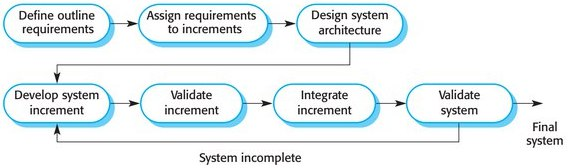
\includegraphics[width=1.0\textwidth, keepaspectratio]{CicloIncrementale.png}
    \caption{Ciclo di vita incrementale}
  \end{center}
\end{figure}
\section{Scadenze}
Le attività di pianificazione del progetto saranno basate sulle scadenze qui riportate:
\begin{itemize}
\item {Revisione dei Requisiti (RR): 2016-02-16;}
\item {Revisione di Progetto (RP): 2016-04-18;}
\item {Revisione di Qualifica (RQ): 2016-05-23;}
\item {Revisione di Accettazione (RA): 2016-07-11.}
\end{itemize}
Si precisa inoltre che il gruppo intende presentare alla Revisione di Progetto la \textit{Specifica Tecnica} e non la \textit{Definizione di Prodotto}.
\section{Analisi dei rischi}
L'analisi dei rischi ha costituito un'\gloss{attività} critica della pianificazione, in
quanto il gruppo \textit{ScalateKids}, alla sua prima esperienza, ha dovuto pensare agli ipotetici
scenari negativi che possono formarsi col procedere dell'\gloss{attività} di sviluppo.\\
Per avere una analisi dei rischi sempre aggiornata il \textit{Responsabile di Progetto} ha deciso che ogni venti giorni si dovrà tenere un breve \gloss{Brainstorming} atto ad analizzare i rischi che possono incorrere con più probabilità. Per questo motivo questa sezione cambierà continuamente.\\
\subsection{Identificazione del rischio}
Per l'identificazione dei rischi il primo passo è stato un'\gloss{attività} di
\gloss{Brainstorming} suddiviso per categorie di pertinenza, in modo da esplorare
in maniera quanto più generale e ampia possibile i vari aspetti di ogni
possibile scenario, seguito da un'\gloss{attività} di analisi di ogni rischio emerso e
l'impatto che questo avrebbe portato al raggiungimento degli obiettivi preposti
per la conclusione del progetto. Le categorie prese in considerazione sono:
\begin{itemize}
\item\textbf{Logistica;}
\item\textbf{Competenza tecnica;}
\item\textbf{Infrastruttura;}
\item\textbf{Organizzativi.}
\end{itemize}
\subsubsection{Parametri di quantificazione dei rischi}
Per ogni possibile rischio previsto l'analisi ha fornito i seguenti parametri:
\begin{itemize}
\item\textbf{Categoria}: Indica la categoria di appartenenza in cui ricade il
  rischio preso in considerazione;
\item\textbf{Probabilità}: Probabilità statistica che lo scenario indesiderato
  si presenti, può assumere i seguenti valori:
  \begin{itemize}
  \item\textbf{Basso;}
  \item\textbf{Medio;}
  \item\textbf{Alto;}
  \item\textbf{Molto alto.}
  \end{itemize}
\item\textbf{Impatto}: Grado di pericolosità dello scenario indesiderato, può
  assumere i seguenti valori:
  \begin{itemize}
  \item\textbf{Debole;}
  \item\textbf{Medio;}
  \item\textbf{Forte;}
  \item\textbf{Molto Forte.}
  \end{itemize}
\item\textbf{Descrizione}: Una descrizione del caso preso in considerazione;
\item\textbf{Contromisure di mitigazione}: Provvedimenti da attuare in
  previsione del rischio, e/o di mitigazione in caso di bisogno;
\item\textbf{Riscontro}: Riscontri eventuali del rischio e contromisure effettuate per mitigare o annullare il problema.
\end{itemize}
\textbf{Tabella delle probabilità}
\begin{table}[H]
  \centering
  \begin{tabular}{|m{2cm}|m{3cm}|m{3cm}|m{3cm}|m{3cm}|}
    \hline
    & \multicolumn{4}{|c|}{\textbf{Probabilità}}\\
    \hline
    \bf Impatto & \bf Bassa & \bf Media & \bf Alta & \textbf{Molto alta} \\
    \hline
    \bf Molto Forte & \cellcolor{red!50} & \cellcolor{red!50} & \cellcolor{red!50} Definizione di prodotto &\cellcolor{red!50} \\
    \hline
    \bf Forte & \cellcolor{yellow!50}Guasti hardware & \cellcolor{yellow!50}Specifica Tecnica & \cellcolor{red!50} Tecnologia di impiego &\cellcolor{red!50} \\[8pt]
    \hline
    \bf Medio & \cellcolor{green!50} Ambiente di lavoro non omogeneo & \cellcolor{yellow!50}Stime attività &\cellcolor{yellow!50} &\cellcolor{red!50}Inesperienza \\[8pt]
    \hline
    \bf Debole & \cellcolor{green!50}Dissensi tra componenti & \cellcolor{green!50} Analisi Requisiti &\cellcolor{yellow!50}Impegni personali &\cellcolor{yellow!50} \\
    \hline
  \end{tabular} \\
\end{table}
\begin{table}[H]
  \centering
  \caption{Legenda colorazione rischi}
  \begin{tabular}{|c|l|}
    \hline \bf Colore & \bf Legenda \\
    \hline \cellcolor{red! 50} & Rischio non accettabile - riduzione obbligatoria \\
    \hline \cellcolor{yellow! 50} & Rischio medio - considerare una riduzione \\
    \hline \cellcolor{green! 50} & Rischio accettabile \\
    \hline
  \end{tabular}
\end{table}
\begin{table}[H]
  \centering
  \caption{Legenda probabilità di riscontro rischi}
  \begin{tabular}{|c|l|}
    \hline \bf Nome & \bf Probabilità prevista \\
    \hline \textbf{Bassa} & 0\% < p < 25\% \\
    \hline \textbf{Media} & 25\% < p < 50\% \\
    \hline \textbf{Alta} & 50\% < p < 75\% \\
    \hline \textbf{Molto Alta} & p > 75\% \\
    \hline
  \end{tabular}
\end{table}

\paragraph{Impegni personali}
\textbf{Categoria}: Logistica\\
\textbf{Probabilità}: Alta\\
\textbf{Impatto}: Debole\\
\textbf{Descrizione}: Il gruppo può avere problemi a riunirsi fisicamente con la maggior parte dei membri presenti.\\
\textbf{Contromisure di mitigazione}: Il \textit{Responsabile di Progetto} ha stabilito una frequenza di incontri fissa.
Il gruppo ha inoltre creato alcuni canali di comunicazione remota in modo da poter lavorare quanto più possibile in
coordinazione reciproca.\\
\textbf{Riscontro}: Gli impegni personali dovuti in particolar modo a impegni universitari sono stati maggiori 
del previsto durante il periodo relativo alla validazione.\\Questo ha influito anche più del previsto 
facendo saltare la consegna del progetto al gruppo. Pertando il gruppo ha dovuto spostare la consegna del 
progetto in data 5 luglio.\\

\paragraph{Inesperienza}
\textbf{Categoria}: Competenza tecnica\\
\textbf{Probabilità}: Alta\\
\textbf{Impatto}: Forte\\
\textbf{Descrizione}: Il gruppo può rimanere spiazzato dal metodo di lavoro da seguire, l'inesperienza nell'attuazione
di competenze di pianificazione e analisi può portare a rallentamenti nel perseguimento degli obiettivi.\\
\textbf{Contromisure di mitigazione}: I componenti del gruppo si impegneranno a studiare e applicarsi il più possibile
nella pratica delle competenze richieste ed, eventualmente, il \textit{Responsabile} potrà riassegnare alcuni ruoli provvisoriamente
basandosi sui punti deboli e forti dei componenti con maggiori difficoltà a portare a termine la propria \gloss{attività}.\\
\textbf{Riscontro}: Questo rischio, come pensavamo, ha causato qualche problema. Per mitigare questi problemi tutti i membri hanno cercato di studiare le materie di interesse il più possibile. Inoltre discussioni e scambi di idee tra i componenti hanno aiutato nella risoluzione.\\
\label{sub:tecnologie}
\paragraph{Tecnologia di impiego}
\textbf{Categoria}: Competenza tecnica\\
\textbf{Probabilità}: Alta\\
\textbf{Impatto}: Forte\\
\textbf{Descrizione}: Le tecnologie impiegate nello sviluppo del progetto poggiano su principi noti in buona misura a tutti
i componenti del gruppo, tuttavia l'assenza di un grado di specializzazione tangibile può generare lacune anche gravi nell'utilizzo
degli strumenti in questione.\\
\textbf{Contromisure di mitigazione}: Ciascun componente del gruppo avrà il compito di documentarsi costantemente e applicarsi
nell'uso delle tecnologie del progetto.\\
\textbf{Riscontro}: L'ingresso di nuove tecnologie di impiego ha portato qualche ritardo.
Tuttavia dopo uno studio da parte dei membri del gruppo sulle tecnologie adottate esse non hanno più causato grandi ritardi.\\

\paragraph{Ambiente di lavoro omogeneo}
\textbf{Categoria}: Infrastruttura\\
\textbf{Probabilità}: Alta\\
\textbf{Impatto}: Debole\\
\textbf{Descrizione}: La quantità di strumenti da utilizzare e la loro grande versatilità, oltre a renderli potenti, genera anche
la necessità di un ambiente di lavoro quanto più omogeneo possibile, in modo da semplificare lo sviluppo e avere un comportamento
da parte delle macchine il più comune possibile, in modo da garantire eventualmente anche la riproducibilità di \gloss{bug} che possono
insorgere.\\
\textbf{Contromisure di mitigazione}: Il gruppo ha deciso di risolvere il problema utilizzando una macchina virtuale
preimpostata per l'utilizzo delle tecnologie inerenti al progetto per l'\gloss{attività} di sviluppo.\\
\textbf{Riscontro}: Il gruppo si è impegnato molto per l'installazione e l'uso di un ambiente uniforme tra tutti (come da \href{run:../Interni/NormeDiProgetto\_v4.0.0.pdf}{Norme Di Progetto v4.0.0}). Questo impegno è stato premiato non riscontrando mai questo tipo di problema.\\

\paragraph{Guasti hardware}
\textbf{Categoria}: Infrastruttura\\
\textbf{Probabilità}: Bassa\\
\textbf{Impatto}: Forte\\
\textbf{Descrizione}: Buona parte del lavoro poggia su server privato gestito dall'\textit{Amministratore} su direttive del \textit{Responsabile},
questo garantisce un buon grado di controllo, ma allo stesso tempo espone a maggiori rischi legati alla natura ``personalizzata'' dell'ambiente di lavoro.\\
\textbf{Contromisure di mitigazione}: Verranno eseguiti dei backup automatici schedulati con periodicità fissa.\\
\textbf{Riscontro}: 
Si è verificato in un paio di occasioni questo tipo di problema, fortunatamente guasti ad un computer personale di un membro del gruppo e non al server privato.\\Un computer di un membro del gruppo ha smesso di funzionare. Questo non ha causato grossi disagi poiché questa persona è ricorsa all'uso del laboratorio informatico in Paolotti per la durata del periodo in cui era sprovvisto del suo computer.

\paragraph{Analisi dei requisiti}
\textbf{Categoria}: Competenza tecnica\\
\textbf{Probabilità}: Medio\\
\textbf{Impatto}: Debole\\
\textbf{Descrizione}: La forte inesperienza del gruppo può portare ad una analisi dei requisiti superficiale o addirittura errata. Questo avrebbe un impatto molto negativo sul progetto.\\Una stesura di requisiti superficiale potrebbe inoltre portare ad una accettazione di requisiti opzionali maggiore di ciò che il gruppo riuscirà a produrre.\\
\textbf{Contromisure di mitigazione:} Verranno effettuate molte \gloss{attività} di \gloss{Brainstorming} per avere i requisiti più precisi possibili. Per questo scopo verranno inoltre organizzati degli incontri con il \textit{Proponente}.\\
\textbf{Riscontro}: Dato che questo documento era già stato sottoposto a tre revisioni prima dell'inizio di questo ultimo periodo esso non ha causato ritardi.\\

\paragraph{Stime di attività}
\textbf{Categoria}: Competenza tecnica\\
\textbf{Probabilità}: Media\\
\textbf{Impatto}: Medio\\
\textbf{Descrizione}: Una cattiva stima delle \gloss{attività} per inesperienza dei membri del gruppo potrebbe portare a forti ritardi rispetto al piano stabilito.\\
\textbf{Contromisure di mitigazione:} Il \textit{Responsabile} tiene traccia dell'avanzamento delle attività. In tal modo potrà assegnare più persone alle attività che richiedono più tempo del previsto.\\
\textbf{Riscontro}:
Le stime delle attività non sono state sempre molto precise, tuttavia attuando le contromisure per questo rischio, l'impatto è stato ridotto notevolmente confermando buone tali contromisure.\\ Inoltre si è scelto di essere particolarmente cauti con la pianificazione delle attività relative alla progettazione, cercando di effettuare riunioni interne frequenti per controllare lo stato di avanzamento e se necessario variando le pianificazioni effettuate in precedenza.\\Per quanto riguarda la fase di validazione la stima delle attività è stata 
sufficientemente precisa ma la consegna si è dovuta spostare a causa di diversi impegni per altri esami da parte 
della maggior parte dei membri del gruppo.\\

\paragraph{Dissensi tra componenti}
\textbf{Categoria}: Organizzativa\\
\textbf{Probabilità}: Debole\\
\textbf{Impatto}: Debole\\
\textbf{Descrizione}: Un dissenso tra componenti potrebbe portare a diversi problemi nella realizzazione del prodotto. Tuttavia questo rischio sembra poter avvenire con scarsa probabilità poiché il gruppo sembra unito e pronto a collaborare secondo regole prestabilite.\\
\textbf{Contromisure di mitigazione:} I componenti del gruppo cercheranno di aderire quanto più possibile alle \href{run:../Interni/NormeDiProgetto\_v4.0.0.pdf}{Norme di Progetto v4.0.0.}. Esse sono state redatte cercando di evitare questo problema.\\
\textbf{Riscontro}: Come il gruppo pensava non è mai insorto nessun problema di questo genere.\\

\paragraph{Specifica tecnica}
\textbf{Categoria}: Competenza tecnica\\
\textbf{Probabilità}: Media\\
\textbf{Impatto}: Forte\\
\textbf{Descrizione}: La forte inesperienza del gruppo può aver portato ad una progettazione architetturale superficiale o addirittura errata. Questo avrebbe un impatto molto negativo sul progetto.\\Una progettazione errata può portare ingenti ritardi al gruppo, causando la riprogettazione delle componenti errati.\\
\textbf{Contromisure di mitigazione:} Verranno effettuate molte \gloss{attività} di \gloss{Brainstorming} per cercare di confermare l'architettura. Per questo scopo verranno inoltre organizzati degli incontri con il \textit{Proponente}.\\
\textbf{Riscontro}: Il documento di specifica tecnica dopo le migliorie dello scorso periodo non ha causato grossi problemi.\\

\paragraph{Definizione di prodotto}
\textbf{Categoria}: Competenza tecnica\\
\textbf{Probabilità}: Alta\\
\textbf{Impatto}: Molto forte\\
\textbf{Descrizione}: La forte inesperienza del gruppo può aver portato ad una progettazione architetturale delle classi superficiale o addirittura errata. Questo avrebbe un impatto molto negativo sul progetto.\\Una progettazione errata può portare ingenti ritardi al gruppo, causando la riprogettazione delle componenti errati.\\
\textbf{Contromisure di mitigazione:} Verranno effettuate molte \gloss{attività} di \gloss{Brainstorming} per cercare di confermare l'architettura. Per questo scopo verranno inoltre organizzati degli incontri con il \textit{Proponente}.\\
\textbf{Riscontro}: Il documento ha dovuto subire forti modifiche per analizzare più approfonditamente le classi, questo ha causato un lieve ritardo nelle attività.\\

\section{Pianificazione}
\subsection{Suddivisione attività}
\label{sub:fasi}
Per semplificare la pianificazione del prospetto orario, sono state identificate
quattro fasi principali che rappresentano l'intero ciclo di sviluppo del prodotto.\\
Esse sono:
\begin{itemize}
\item\textbf{Analisi (AN):} rappresenta il primo periodo del progetto,
dalla
  pubblicazione dei capitolati d'appalto all'inizio dell'\gloss{attività} di progettazione.\\
  Figure maggiormente coinvolte: \textit{Responsabile, Amministratore, Analista, Verificatore};
\item\textbf{Analisi di Dettaglio (AD) e Progettazione Architetturale (PA):} segue la fase di Analisi, e
  racchiude il lasso temporale dedicato alla correzione degli errori rilevati in
  sede di Revisione di Requisiti e alla progettazione dell'architettura sulla
  base dei requisiti emersi. Comprende anche lo studio di \gloss{design pattern}
  congrui alla realizzazione del prodotto.\\ Figure maggiormente coinvolte:
  \textit{Responsabile, Amministratore, Progettista, Verificatore};
\item\textbf{Progettazione di Dettaglio (PD) e Codifica(C):} comprende la correzione degli errori rilevati in sede di Revisione di Progettazione, la progettazione di dettaglio e la stesura del \gloss{codice} secondo le direttive emerse durante l'\gloss{attività} di progettazione.\\Figure maggiormente coinvolte:
  \textit{Responsabile, Amministratore, Progettista, Programmatore, Verificatore};
\item\textbf{Validazione (VV):} in questa fase si andranno a correggere eventuali errori emersi in Revisione di Qualifica e si finirà il prodotto in tutti i suoi componenti per poi fare il collaudo finale col \textit{Proponente}.
\end{itemize}
Tutte le fasi descritte sono comprensive di numerose \gloss{attività} di \textbf{Verifica}, in quanto necessaria durante tutto l'arco di sviluppo del prodotto.\\Ogni \gloss{attività} prevede l'impiego di alcuni ruoli in misura maggiore rispetto ad altri, nella distribuzione di questi sarà garantita un equa ripartizione del
carico di lavoro individuale.\\
Come riportato nelle \href{run:../Interni/NormeDiProgetto\_v4.0.0.pdf}{Norme Di Progetto v4.0.0} ogni componente del gruppo potrà ricoprire più ruoli contemporaneamente, purché sia garantita l'assenza di conflitti d'interesse tra le \gloss{attività} svolte.\\ \\
\textbf{Diagrammi di Gantt}\\
Sono riportati nei prossimi capitoli i \gloss{diagrammi di Gantt} relativi alle fasi elencate e un \gloss{diagramma di Gantt} preventivo di tutto l'arco temporale previsto per la realizzazione del prodotto.\\
Nei \gloss{diagrammi di Gantt} verranno riportati diversi elementi importanti:
\begin{itemize}
\item \textbf{Attività composta:} riportata con barra nera nei diagrammi indica una marco-\gloss{attività} composta in più \gloss{attività} minori riportate al di sotto di essa;
\item \textbf{Attività non critica:} riportata con barra blu nei diagrammi indica una \gloss{attività} che può essere svolta parallelamente a altre \gloss{attività}. Un ritardo su un'\gloss{attività} di questo tipo non causerebbe ritardi a cascata su altre \gloss{attività};
\item \textbf{Attività critica:} riportata con una barra arancio nei diagrammi indica un'\gloss{attività} che ha un forte impatto temporale nello svolgersi del progetto, pertanto un ritardo in un'\gloss{attività} di questo tipo causerebbe un ritardo a cascata nel resto del progetto impattando negativamente il piano temporale ed economico;
\item \textbf{Milestone:} riportata con un rombo nero nei diagrammi indica la data attesa per la conclusione delle \gloss{attività}. Coincide con la consegna del prodotto e documenti della successiva revisione.
\end{itemize}
\subsubsection{Tabelle di distribuzione dei ruoli}
Per semplificare la rappresentazione della distribuzione ore/ruoli durante il
progetto sono state raggruppate le ore con investimento e le ore rendicontate. Per ore rendicontate si intendono le ore di lavoro effettive, le ore con investimento rappresentano le ore rendicontate sommate a delle ore di slack. Dal totale si ricava che c'è uno slack medio totale del 18\%. \\ \\
\textbf{Legenda:}
\begin{itemize}
\item\textbf{Res:} \textit{Responsabile di Progetto};
\item\textbf{An:} \textit{Analista};
\item\textbf{Amm:} \textit{Amministratore};
\item\textbf{Pr:} \textit{Progettista};
\item\textbf{Pt:} \textit{Programmatore};
\item\textbf{Ve:} \textit{Verificatore}
\item\textbf{Inv:} Ore con investimento;
\item\textbf{Ren:} Ore con rendicontazione.
\end{itemize}
\subsubsection{Analisi}
Nell'\gloss{attività} di Analisi, i componenti ricopriranno i ruoli di progetto secondo la distribuzione seguente:
\begin{center}
  \scriptsize
  \begin{tabular}{| c | p{0.35cm} p{0.35cm} | p{0.35cm} p{0.35cm} | p{0.35cm} p{0.35cm} | p{0.35cm} p{0.35cm} | p{0.35cm} p{0.35cm} | p{0.35cm} p{0.35cm} | p{0.35cm} p{0.35cm} |}
    \hline
    \textbf{Nome} & \multicolumn{2}{|c|}{\textbf{Res}} & \multicolumn{2}{|c|}{\textbf{An}} & \multicolumn{2}{|c|}{\textbf{Amm}} & \multicolumn{2}{|c|}{\textbf{Pr}} & \multicolumn{2}{|c|}{\textbf{Pt}} & \multicolumn{2}{|c|}{\textbf{Ve}} & \multicolumn{2}{|c|}{\textbf{Tot}}\\
    \hline
    & \textbf{Inv} & \textbf{Ren} & \textbf{Inv} & \textbf{Ren} & \textbf{Inv} & \textbf{Ren} & \textbf{Inv} & \textbf{Ren} & \textbf{Inv} & \textbf{Ren} & \textbf{Inv} & \textbf{Ren} & \textbf{Inv} & \textbf{Ren}\\
    \hline
    Andrea Baldan & 12 & 10 & & & 10 & 8 & & & & & 12 & 9 & 34 & 27\\
    Alberto de Agostini & 12 & 9 & 12 & 10 & & & & & & & 18 & 15 & 42 & 34\\
    Michael Munaro & & & 14 & 12 & & & & & & & 16 & 14 & 30 & 26\\
    Giacomo Vanin & & & 14 & 12 & & & & & & & 19 & 16 & 33 & 28\\
    Marco Boseggia & & & 14 & 12 & & & & & & & 16 & 15 & 30 & 27\\
    Francesco Agostini & & & 5 & 4 & 10 & 8 & & & & & 14 & 12 & 29 & 24\\
    Davide Trevisan & & & 14 & 12 & & & & & & & 16 & 13 & 30 & 25\\
    \hline
  \end{tabular}
\end{center}
I seguenti grafici illustrano le ore investite per Persona suddivise tra ore investite e ore rendicontate, per l'\gloss{attività} di Analisi.
\begin{figure}[H]
  \begin{subfigure}[H]{0.47\textwidth}
    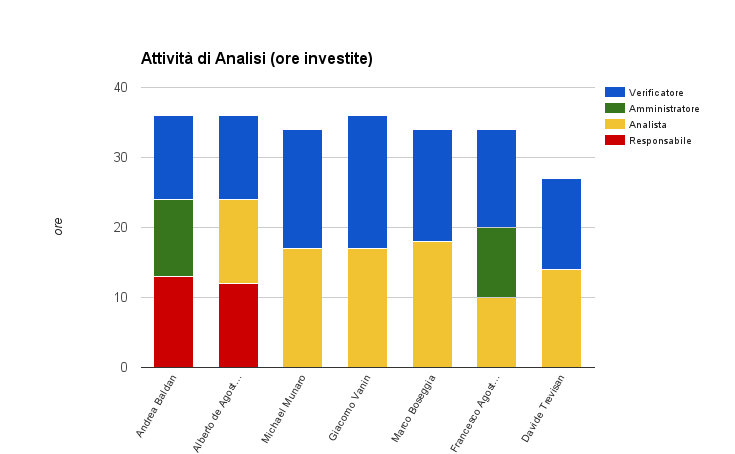
\includegraphics[width=1.2\textwidth,keepaspectratio]{AnalisiConInvestimento.png}
    \caption{Ore con investimento, \gloss{attività} di Analisi}
  \end{subfigure}
  \qquad
  \begin{subfigure}[H]{0.47\textwidth}
    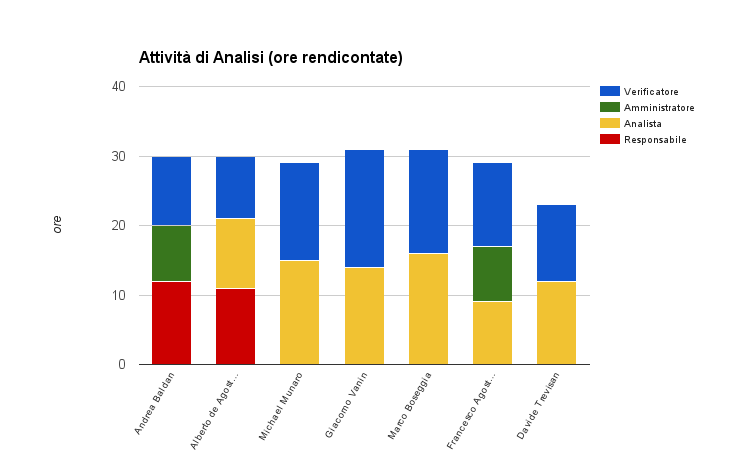
\includegraphics[width=1.2\textwidth,keepaspectratio]{AnalisiConRendicontazione.png}
    \caption{Ore con rendicontazione, \gloss{attività} di Analisi}
  \end{subfigure}
\end{figure}

\newpage
\paragraph{Pianificazione temporale}
\begin{figure}[H]
  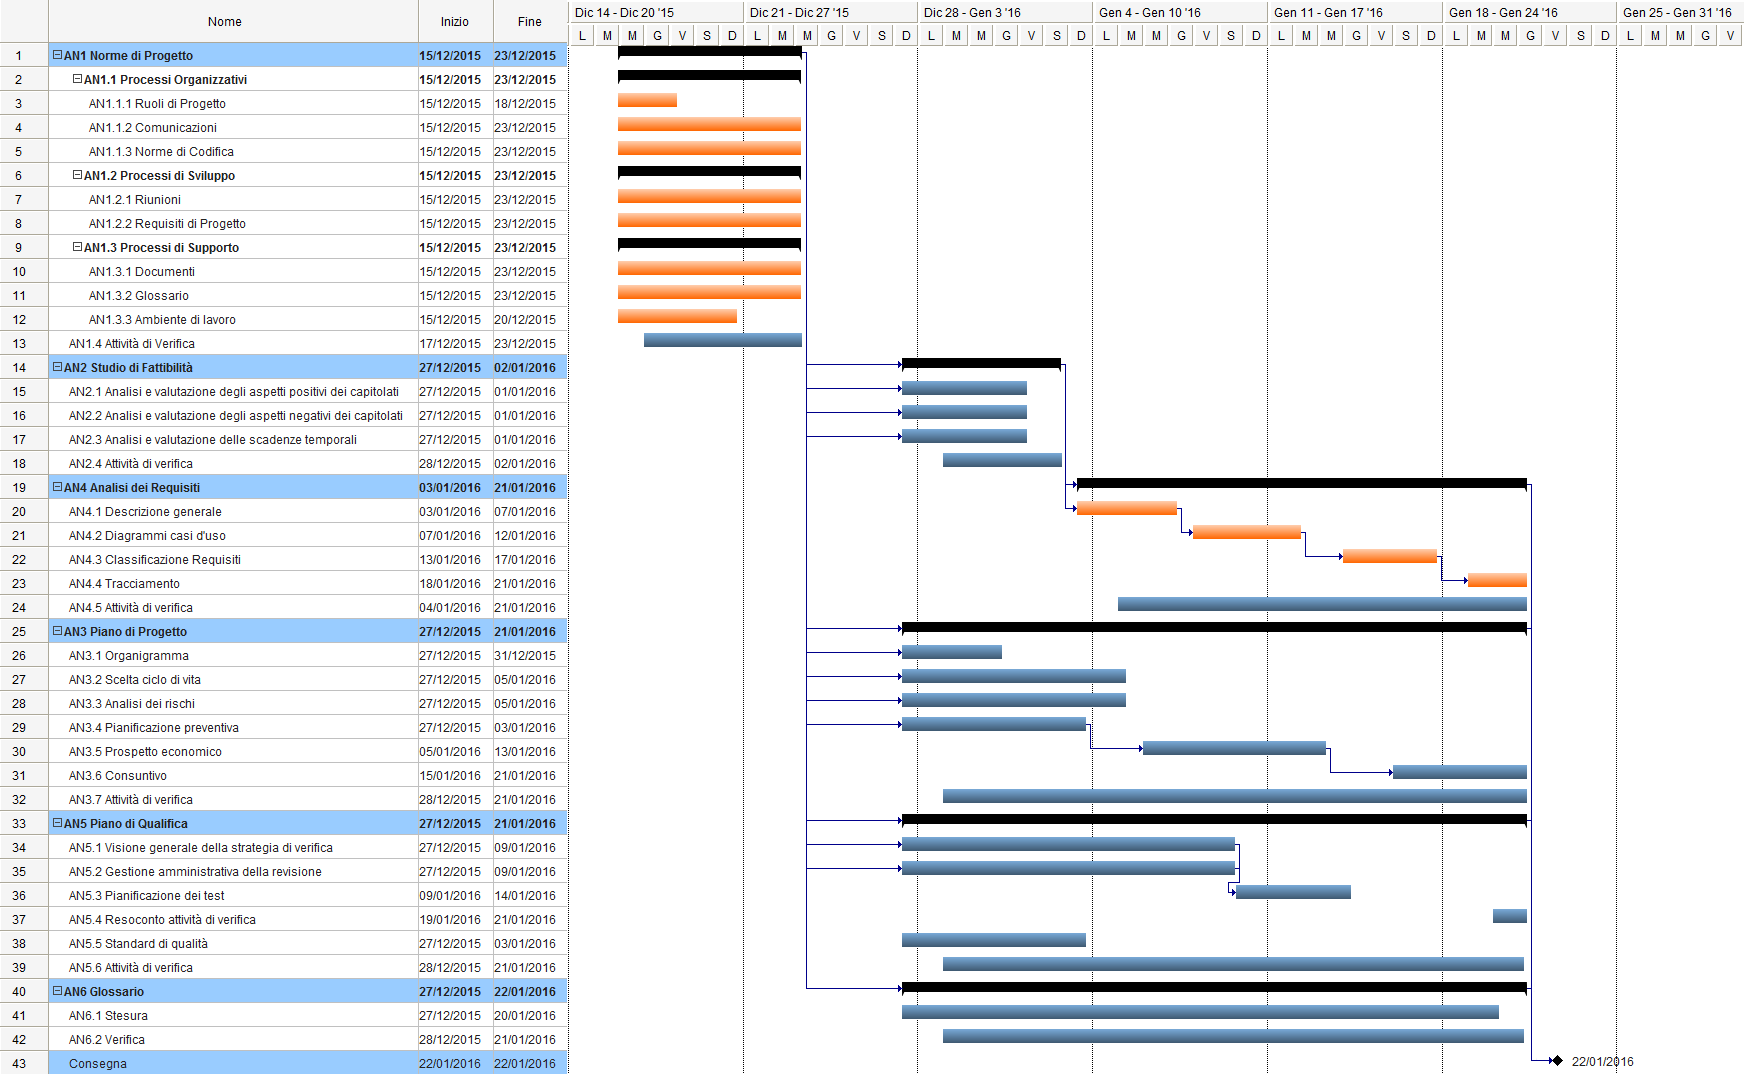
\includegraphics[width=1.0\textwidth, keepaspectratio]{gantt/1-Revisione-Requisiti-gantt-preventivo.png}
  \caption{Gantt preventivo delle \gloss{attività} di Analisi}
\end{figure}

\newpage
\textbf{Distribuzione oraria}
\scriptsize
\begin{center}
  \begin{tabular}{| c | c | c | c |}
    \hline
    \textbf{Id} & \textbf{Nome} & \textbf{Ruolo} & \textbf{Ore}\\
    \hline
    \textbf{AN1} & \textbf{Norme di Progetto} & &\\
    \hline
    \textit{AN1.1} & \textit{Processi organizzativi} & &\\
    \hline
    AN1.1.1 & Ruoli di progetto & Amministratore 1 & 1\\
    \hline
    AN1.1.2 & Comunicazioni & Amministratore 1 & 2\\
    \hline
    AN1.1.3 & Norme di Codifica & Amministratore 2 & 3\\
    \hline
    \textit{AN1.2} & \textit{Processi di Sviluppo} & &\\
    \hline
    AN1.2.1 & Riunioni & Amministratore 2 & 2\\
    \hline
    AN1.2.2 & Requisiti di Progetto & Amministratore 1 & 3\\
    \hline
    \textit{AN1.3} & \textit{Processi di Supporto} & &\\
    \hline
    AN1.3.1 & Documenti & Amministratore 1 & 4\\
    \hline
    AN1.3.2 & Glossario & Amministratore 1 & 2\\
    \hline
    AN1.3.3 & Ambiente di Lavoro & Amministratore 2 & 3\\
    \hline
    AN1.4 & Attività di Verifica & \multiLineCell[t]{Verificatore 1\\Verificatore 3} & \multiLineCell[t]{8\\8}\\
    \hline
    \textbf{AN2} & \textbf{Studio di Fattibilità} & &\\
    \hline
    AN2.1 & Analisi e valutazione degli aspetti positivi dei capitolati & Analista 1 & 5\\
    \hline
    AN2.2 & Analisi e valutazione degli aspetti negativi dei capitolati & Analista 2 & 5\\
    \hline
    AN2.3 & Analisi e valutazione delle scadenze temporali & Analista 3 & 5\\
    \hline
    AN2.4 & Attività di verifica & \multiLineCell[t]{Verificatore 2\\Verificatore 4} & \multiLineCell[t]{4\\5}\\
    \hline
    \textbf{AN4} & \textbf{Analisi dei Requisiti} & &\\
    \hline
    AN4.1 & Descrizione Generale & \multiLineCell[t]{Analista 3\\Analista 2} & \multiLineCell[t]{3\\3}\\
    \hline
    AN4.2 & Diagrammi Casi d'uso & \multiLineCell[t]{Analista 4\\Analista 1\\Analista 3} & \multiLineCell[t]{5\\6\\5}\\
    \hline
    AN4.3 & Classificazione Requisiti & \multiLineCell[t]{Analista 3\\Analista 2} & \multiLineCell[t]{3\\4}\\
    \hline
    AN4.4 & Tracciamento & \multiLineCell[t]{Analista 1\\Analista 2\\Analista 3} & \multiLineCell[t]{3\\3\\4}\\
    \hline
    AN4.5 & Attività di Verifica & \multiLineCell[t]{Verificatore 1\\Verificatore 2\\Verificatore 3} & \multiLineCell[t]{9\\10\\9}\\
    \hline
    \textbf{AN3} & \textbf{Piano di Progetto} & &\\
    \hline
    AN3.1 & Organigramma & Responsabile & 2\\
    \hline
    AN3.2 & Scelta ciclo di vita & Responsabile & 4\\
    \hline
    AN3.3 & Analisi dei Rischi & Responsabile & 5\\
    \hline
    AN3.4 & Pianificazione & Responsabile & 5\\
    \hline
    AN3.5 & Prospetto Economico & Responsabile & 2\\
    \hline
    AN3.6 & Consuntivo & Responsabile & 3\\
    \hline
    AN3.7 & Attività di Verifica & \multiLineCell[t]{Verificatore 4\\Verificatore 5} & \multiLineCell[t]{10\\10}\\
    \hline
    \textbf{AN5} & \textbf{Piano di Qualifica} & &\\
    \hline
    AN5.1 & Visione generale della strategia di verifica & \multiLineCell[t]{Responsabile\\Analista 1\\Verificatore 1} & \multiLineCell[t]{3\\5\\4}\\
    \hline
    AN5.2 & Gestione amministrativa della revisione & \multiLineCell[t]{Analista 1\\Analista 2} & \multiLineCell[t]{2\\3}\\
    \hline
    AN5.3 & Pianificazione dei Test & \multiLineCell[t]{Analista 2\\Analista 3} & \multiLineCell[t]{2\\3}\\
    \hline
    AN5.4 & Resoconto Attività di Verifica & Verificatore 4 & 8\\
    \hline
    AN5.5 & Standard di Qualità & Analista 4 & 5\\
    \hline
    AN5.6 & Attività di Verifica & \multiLineCell[t]{Verificatore 1\\Verificatore 3\\Verificatore 5} & \multiLineCell[t]{4\\5\\9}\\
    \hline
    \textbf{AN6} & \textbf{Glossario} & &\\
    \hline
    AN6.1 & Stesura & &\\
    \hline
    AN6.2 & Verifica & Verificatore 1 & 7
  \end{tabular}
\end{center}
\normalsize

\newpage
\subsubsection{Progettazione}
Durante l'\gloss{attività} di Progettazione, i componenti ricopriranno i ruoli di progetto secondo la distribuzione seguente:
\begin{center}
  \scriptsize
  \begin{tabular}{| c | p{0.35cm}  p{0.35cm} | p{0.35cm}  p{0.35cm} | p{0.35cm}  p{0.35cm} | p{0.35cm}  p{0.35cm} | p{0.35cm}  p{0.35cm} | p{0.35cm}  p{0.35cm} | p{0.35cm}  p{0.35cm} |}
    \hline
    \textbf{Nome} & \multicolumn{2}{|c|}{\textbf{Res}} & \multicolumn{2}{|c|}{\textbf{An}} & \multicolumn{2}{|c|}{\textbf{Amm}} & \multicolumn{2}{|c|}{\textbf{Pr}} & \multicolumn{2}{|c|}{\textbf{Pt}} & \multicolumn{2}{|c|}{\textbf{Ve}} & \multicolumn{2}{|c|}{\textbf{Tot}}\\
    \hline
    & \textbf{Inv} & \textbf{Ren} & \textbf{Inv} & \textbf{Ren} & \textbf{Inv} & \textbf{Ren} & \textbf{Inv} & \textbf{Ren} & \textbf{Inv} & \textbf{Ren} & \textbf{Inv} & \textbf{Ren} & \textbf{Inv} & \textbf{Ren}\\
    \hline
    Andrea Baldan & & & 8 & 6 & & & 17 & 14 & & & 12 & 11 & 37 & 31\\
    Alberto de Agostini & & & 6 & 4 & 5 & 5 & 20 & 18 & & & & & 31 & 27\\
    Michael Munaro & & & 7 & 5 & & & & & & & 18 & 15 & 25 & 20\\
    Giacomo Vanin & 11 & 10 & & & & & 18 & 16 & & & & & 29 & 26\\
    Marco Boseggia & 8 & 7 & & & 4 & 3 & 6 & 5 & & & 17 & 15 & 35 & 30\\
    Francesco Agostini & & & 8 & 7 & & & 17 & 15 & & & & & 25 & 22\\
    Davide Trevisan & & & & & & & 16 & 13 & & & 9 & 8 & 25 & 21\\
    \hline
  \end{tabular}
\end{center}
I seguenti grafici illustrano le ore investite per Persona suddivise tra ore
investite e ore rendicontate, per l'\gloss{attività} di Progettazione, comprensive delle
ore riservate all'\gloss{attività} \textbf{Analisi di dettaglio}.
\begin{figure}[H]
  \begin{subfigure}[H]{0.47\textwidth}
    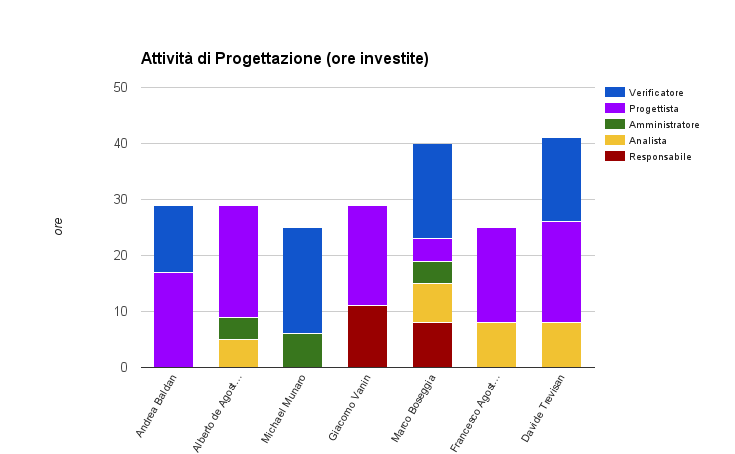
\includegraphics[width=1.2\textwidth,keepaspectratio]{ProgettazioneConInvestimento.png}
    \caption{Ore con investimento, \gloss{attività} di Progettazione}
  \end{subfigure}
  \qquad
  \begin{subfigure}[H]{0.47\textwidth}
    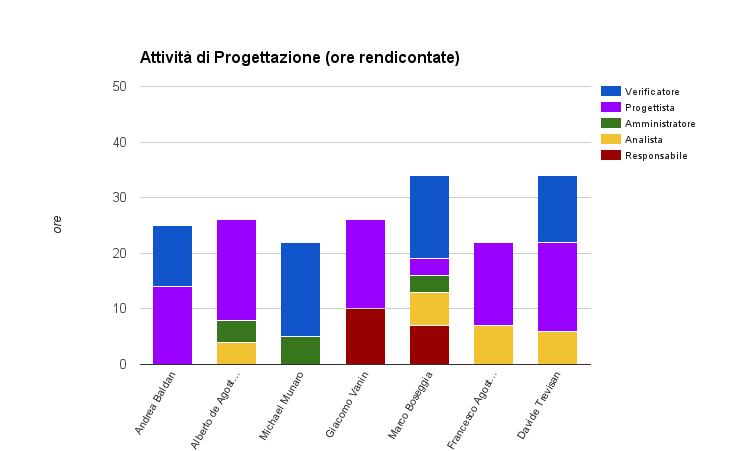
\includegraphics[width=1.2\textwidth,keepaspectratio]{ProgettazioneConRendicontazione.png}
    \caption{Ore con rendicontazione, \gloss{attività} di Progettazione}
  \end{subfigure}
\end{figure}

\newpage
\paragraph{Pianificazione temporale}
\begin{figure}[H]
  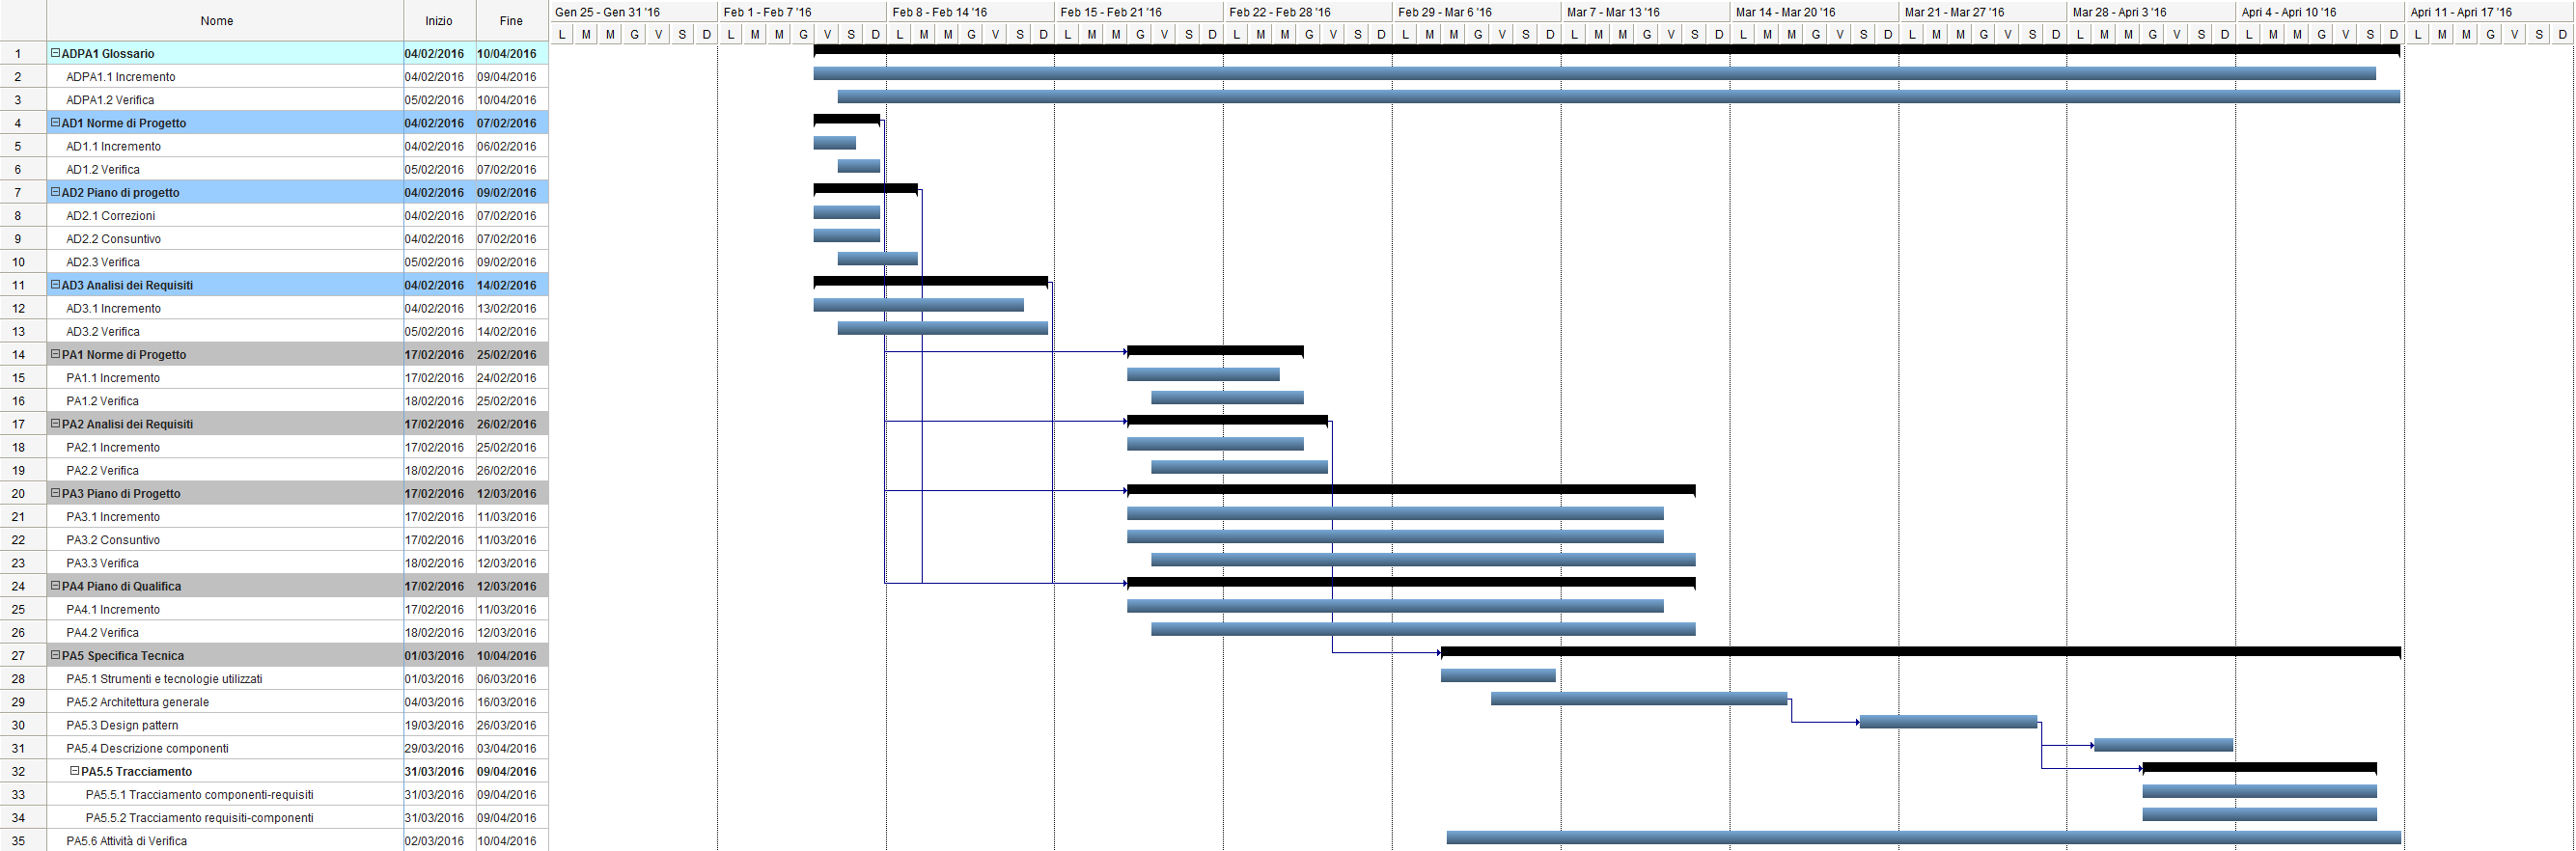
\includegraphics[width=1.0\textwidth, keepaspectratio]{gantt/2-Revisione-Progettazione-gantt-preventivo.png}
  \caption{Gantt preventivo delle \gloss{attività} di Progettazione}
\end{figure}

\newpage
\textbf{Distribuzione oraria}
\scriptsize
\begin{center}
  \begin{tabular}{| c | c | c | c |}
    \hline
    \textbf{Id} & \textbf{Nome} & \textbf{Ruolo} & \textbf{Ore}\\
    \hline
    \textbf{ADPA1} & \textbf{Glossario} & &\\
    \hline
    ADPA1.1 & Incremento &  &\\
    \hline
    ADPA1.2 & Verifica & Verificatore 1 & 4\\
    \hline
    \textbf{AD1} & \textbf{Norme di Progetto} & &\\
    \hline
    AD1.1 & Incremento & \multiLineCell[t]{Amministratore 1\\Amministratore 2} & \multiLineCell[t]{2\\2}\\
    \hline
    AD1.2 & Verifica & Verificatore 2 & 4\\
    \hline
    \textbf{AD2} & \textbf{Piano di Progetto} & &\\
    \hline
    AD2.1 & Correzioni & Responsabile & 5\\
    \hline
    AD2.2 & Consuntivo & Responsabile & 4\\
    \hline
    AD2.3 & Verifica & Verificatore 3 & 6\\
    \hline
    \textbf{AD3} & \textbf{Analisi dei Requisiti} & &\\
    \hline
    AD3.1 & Incremento & \multiLineCell[t]{Analista 1\\Analista 2} & \multiLineCell[t]{4\\4}\\
    \hline
    AD3.2 & Verifica & Verificatore 1 & 4\\
    \hline
    \textbf{PA1} & \textbf{Norme di Progetto} & &\\
    \hline
    PA1.1 & Incremento & \multiLineCell[t]{Amministratore 1\\Amministratore 2} & \multiLineCell[t]{2\\2}\\
    \hline
    PA1.2 & Verifica & Verificatore 2 & 3\\
    \hline
    \textbf{PA2} & \textbf{Analisi dei Requisiti} & &\\
    \hline
    PA2.1 & Incremento & Analista 3 & 6\\
    \hline
    PA2.2 & Verifica & Verificatore 3 & 4\\
    \hline
    \textbf{PA3} & \textbf{Piano di Progetto} & &\\
    PA3.1 & Incremento & Responsabile & 4\\
    \hline
    PA3.2 & Consuntivo & Responsabile & 4\\
    \hline
    PA3.3 & Verifica & Verificatore 1 & 4\\
    \hline
    \textbf{PA4} & \textbf{Piano di Qualifica} & &\\
    \hline
    PA4.1 & Incremento & \multiLineCell[t]{Responsabile\\Progettista 1\\Analista 3} & \multiLineCell[t]{2\\2\\3}\\
    \hline
    PA4.2 & Verifica & \multiLineCell[t]{Verificatore 1\\Verificatore 2} & \multiLineCell[t]{4\\4}\\
    \hline
    \textbf{PA5} & \textbf{Specifica Tecnica} & &\\
    \hline
    PA5.1 & Strumenti e tecnologie usati & \multiLineCell[t]{Amministratore 1\\Progettista 1} & \multiLineCell[t]{1\\6}\\
    \hline
    PA5.2 & Architettura generale & \multiLineCell[t]{Progettista 2\\Progettista 3\\Progettista 4} & \multiLineCell[t]{7\\7\\7}\\
    \hline
    PA5.3 & Design pattern & \multiLineCell[t]{Progettista 1\\Progettista 2\\Progettista 3} & \multiLineCell[t]{8\\6\\7}\\
    \hline
    PA5.4 & Descrizione componenti & \multiLineCell[t]{Progettista 1\\Progettista 2\\Progettista 3\\Progettista 4} & \multiLineCell[t]{8\\8\\8\\8}\\
    \hline
    \textit{PA5.5} & \textit{Tracciamento} &  &\\
    \hline
    PA5.5.1 & Tracciamento componenti-requisiti & \multiLineCell[t]{Analista 1\\Progettista 4} & \multiLineCell[t]{10\\10}\\
    \hline
    PA5.5.2 & Tracciamento requisiti-componenti & \multiLineCell[t]{Analista 2\\Progettista 3} & \multiLineCell[t]{2\\2}\\
    \hline
    PA5.6 & Attività di verifica & \multiLineCell[t]{Verificatore 3\\Verificatore 1} & \multiLineCell[t]{10\\9}\\
    \hline
  \end{tabular}
\end{center}
\normalsize


\subsubsection{Codifica}
Durante l'\gloss{attività} di Codifica, i componenti ricopriranno i ruoli di progetto secondo la distribuzione seguente:
\begin{center}
  \scriptsize
  \begin{tabular}{| c | p{0.35cm}  p{0.35cm} | p{0.35cm}  p{0.35cm} | p{0.35cm}  p{0.35cm} | p{0.35cm}  p{0.35cm} | p{0.35cm}  p{0.35cm} | p{0.35cm}  p{0.35cm} | p{0.35cm}  p{0.35cm} |}
    \hline
    \textbf{Nome} & \multicolumn{2}{|c|}{\textbf{Res}} & \multicolumn{2}{|c|}{\textbf{An}} & \multicolumn{2}{|c|}{\textbf{Amm}} & \multicolumn{2}{|c|}{\textbf{Pr}} & \multicolumn{2}{|c|}{\textbf{Pt}} & \multicolumn{2}{|c|}{\textbf{Ve}} & \multicolumn{2}{|c|}{\textbf{Tot}}\\
    \hline
    & \textbf{Inv} & \textbf{Ren} & \textbf{Inv} & \textbf{Ren} & \textbf{Inv} & \textbf{Ren} & \textbf{Inv} & \textbf{Ren} & \textbf{Inv} & \textbf{Ren} & \textbf{Inv} & \textbf{Ren} & \textbf{Inv} & \textbf{Ren}\\
    \hline
    Andrea Baldan & & & 7 & 6 & & & 17 & 15 & 14 & 12 & & & 38 & 33\\
    Alberto de Agostini & & & & & & & 14 & 11 & 14 & 12 & 16 & 12 & 44 & 35\\
    Michael Munaro & 10 & 9 & & & & & 18 & 15 & 14 & 11 & 15 & 12 & 57 & 47\\
    Giacomo Vanin & & & & & 6 & 5 & & & 20 & 18 & 24 & 18 & 50 & 41\\
    Marco Boseggia & & & & & & & 19 & 16 & 17 & 15 & & & 36 & 31\\
    Francesco Agostini & 8 & 7 & & & & & 18 & 16 & 10 & 9 & 20 & 18 & 56 & 50\\
    Davide Trevisan & & & & & 4 & 3 & 17 & 15 & 16 & 14 & 16 & 14 & 53 & 46\\
    \hline
  \end{tabular}
\end{center}
\normalsize I seguenti grafici illustrano le ore investite per Persona suddivise
tra ore investite e ore rendicontate, per l'\gloss{attività} di Codifica, comprensive
delle ore riservate per l'\gloss{attività} \textbf{Progettazione di Dettaglio}.
\begin{figure}[H]
  \begin{subfigure}[H]{0.47\textwidth}
    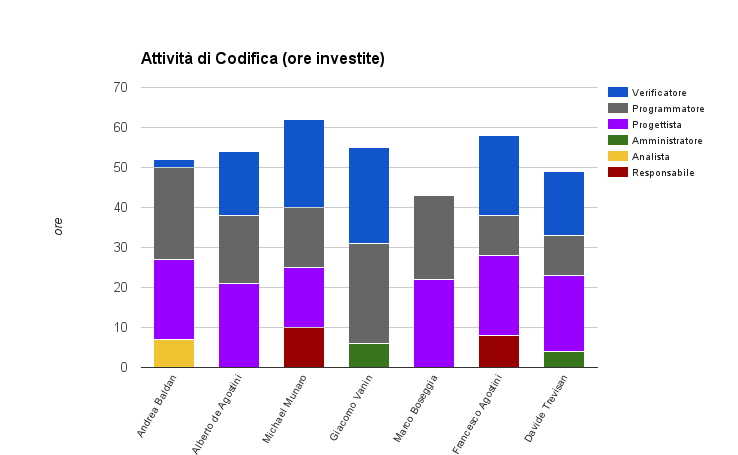
\includegraphics[width=1.2\textwidth,keepaspectratio]{CodificaConInvestimento.png}
    \caption{Ore con investimento, \gloss{attività} di Codifica}
  \end{subfigure}
  \qquad
  \begin{subfigure}[H]{0.47\textwidth}
    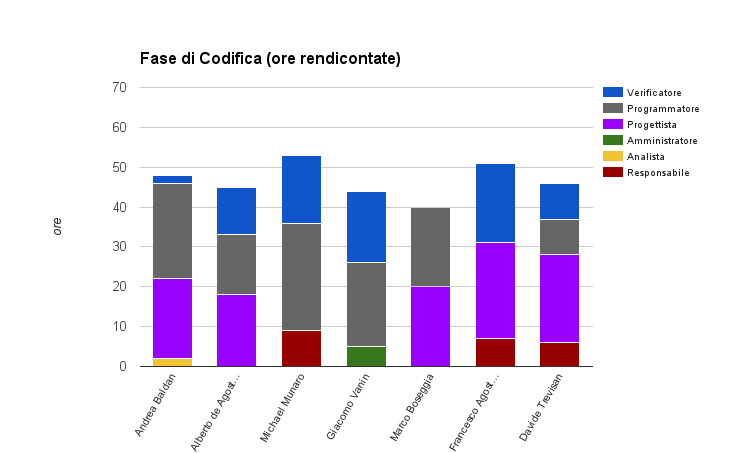
\includegraphics[width=1.2\textwidth,keepaspectratio]{CodificaConRendicontazione.png}
    \caption{Ore con rendicontazione, \gloss{attività} di Codifica}
  \end{subfigure}
\end{figure}

\newpage
\paragraph{Pianificazione temporale}
\begin{figure}[H]
  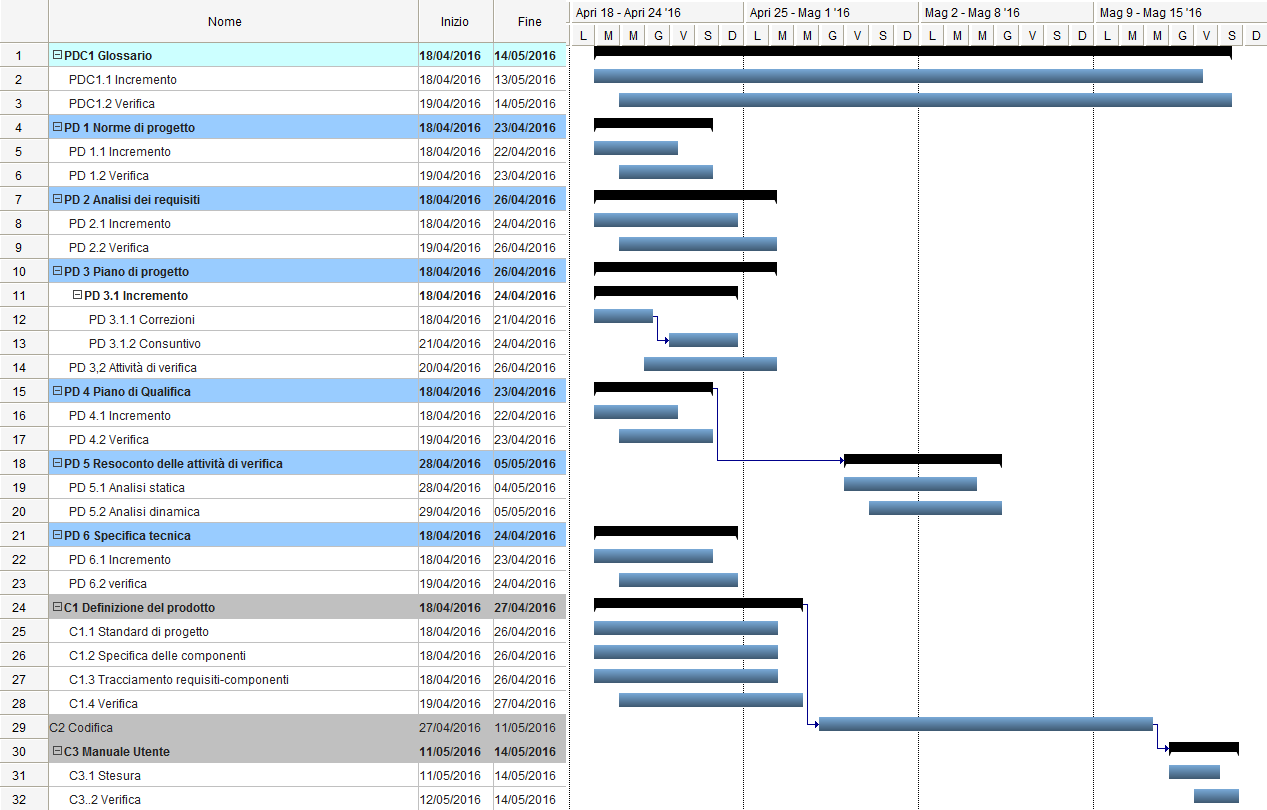
\includegraphics[width=1.0\textwidth, keepaspectratio]{gantt/3-Revisione-Qualifica-gantt-preventivo.png}
  \caption{Gantt preventivo delle \gloss{attività} di codifica}
\end{figure}

\newpage
\textbf{Distribuzione oraria}
\scriptsize
\begin{center}
  \begin{tabular}{| c | c | c | c |}
    \hline
    \textbf{Id} & \textbf{Nome} & \textbf{Ruolo} & \textbf{Ore}\\
    \hline
    \textbf{PDC1} & \textbf{Glossario} & &\\
    \hline
    PDC1.1 & Incremento &  &\\
    \hline
    PDC1.2 & Verifica & Verificatore 1 & 1\\
    \hline
    \textbf{PD1} & \textbf{Norme di Progetto} & &\\
    \hline
    PD1.1 & Incremento & Amministratore 1 & 3\\
    \hline
    PD1.2 & Verifica & Verificatore 2 & 2\\
    \hline
    \textbf{PD2} & \textbf{Analisi dei Requisiti} & &\\
    \hline
    PD2.1 & Incremento & Analista 1 & 3\\
    \hline
    AD2.3 & Verifica & Verificatore 3 & 2\\
    \hline
    \textbf{PD3} & \textbf{Piano di Progetto} & &\\
    \hline
    \textit{PD3.1} & \textit{Incremento} & &\\
    \hline
    PD3.1.1 & Correzioni & Responsabile & 2\\
    \hline
    PD3.1.2 & Consuntivo & Responsabile & 2\\
    \hline
    PD3.2 & Attività di Verifica & Verificatore 1 & 2\\
    \hline
    \textbf{PD4} & \textbf{Piano di Qualifica} & &\\
    \hline
    PD4.1 & Incremento & \multiLineCell[t]{Verificatore 3\\Progettista 1} & \multiLineCell[t]{3\\5}\\
    \hline
    PD4.2 & Verifica & \multiLineCell[t]{Verificatore 2\\Verificatore 3} & \multiLineCell[t]{2\\2}\\
    \hline
    \textbf{PD5} & \textbf{Resoconto delle \gloss{attività} di verifica} & &\\
    \hline
    PD5.1 & Analisi statica & Verificatore 1 & 7\\
    \hline
    PD5.2 & Analisi dinamica & Verificatore 2 & 7\\
    \hline
    \textbf{PD6} & \textbf{Specifica Tecnica} & &\\
    \hline
    PD6.1 & Incremento & Progettista 2 & 5\\
    \hline
    PD6.2 & Verifica & Verificatore 3 & 3\\
    \hline
    \textbf{C1} & Definizione del Prodotto & &\\
    \hline
    C1.1 & Standard di progetto & \multiLineCell[t]{Progettista 3\\Progettista 4} & \multiLineCell[t]{14\\14}\\
    \hline
    C1.2 & Specifica delle componenti & \multiLineCell[t]{Progettista 1\\Progettista 2} & \multiLineCell[t]{14\\14}\\
    \hline
    C1.3 & Tracciamento requisiti-componenti & \multiLineCell[t]{Progettista 2\\Progettista 2} & \multiLineCell[t]{14\\14}\\
    \hline
    C1.4 & Verifica & \multiLineCell[t]{Verificatore 1\\Verificatore 2\\Verificatore 3} & \multiLineCell[t]{10\\10\\10}\\
    \hline
    \textbf{C2} & \textbf{Codifica} & \multiLineCell[t]{Programmatore 1\\Programmatore 2\\Programmatore 3\\Programmatore 4\\Verificatore 1\\Verificatore 2\\Verificatore 3} & \multiLineCell[t]{26\\27\\26\\26\\10\\10\\10}\\
    \hline
    \textbf{C3} & \textbf{Manuale Utente} & &\\
    \hline
    C3.1 & Stesura & \multiLineCell[t]{Amministratore\\Analista\\Responsabile} & \multiLineCell[t]{7\\4\\7}\\
    \hline
    C3.2 & Verifica & Responsabile & 16\\
    \hline
  \end{tabular}
\end{center}
\normalsize
\newpage

\subsubsection{Validazione}
Durante le \gloss{attività} di validazione, i componenti ricopriranno i ruoli di progetto secondo la distribuzione seguente:
\begin{center}
  \scriptsize
  \begin{tabular}{| c | p{0.35cm}  p{0.35cm} | p{0.35cm}  p{0.35cm} | p{0.35cm}  p{0.35cm} | p{0.35cm}  p{0.35cm} | p{0.35cm}  p{0.35cm} | p{0.35cm}  p{0.35cm} | p{0.35cm}  p{0.35cm} |}
    \hline
    \textbf{Nome} & \multicolumn{2}{|c|}{\textbf{Res}} & \multicolumn{2}{|c|}{\textbf{An}} & \multicolumn{2}{|c|}{\textbf{Amm}} & \multicolumn{2}{|c|}{\textbf{Pr}} & \multicolumn{2}{|c|}{\textbf{Pt}} & \multicolumn{2}{|c|}{\textbf{Ve}} & \multicolumn{2}{|c|}{\textbf{Tot}}\\

    \hline
    & \textbf{Inv} & \textbf{Ren} & \textbf{Inv} & \textbf{Ren} & \textbf{Inv} & \textbf{Ren} & \textbf{Inv} & \textbf{Ren} & \textbf{Inv} & \textbf{Ren} & \textbf{Inv} & \textbf{Ren} & \textbf{Inv} & \textbf{Ren}\\
    \hline
    Andrea Baldan & & & & & & & 4 & 4 & 8 & 6 & & & 12 & 10\\
    Alberto de Agostini & & & & & & & 4 & 3 & 3 & 3 & & & 7 & 6\\
    Michael Munaro & & & & & 6 & 5 & & & & & 7 & 6 & 13 & 11\\
    Giacomo Vanin & & & 4 & 3 & & & & & 5 & 4 & & & 9 & 7\\
    Marco Boseggia & & & 6 & 4 & & & 4 & 3 & & & 6 & 5 & 16 & 12\\
    Francesco Agostini & & & 6 & 5 & & & 2 & 2 & & & & & 8 & 7\\
    Davide Trevisan & 6 & 6 & & & & & & & 5 & 4 & & & 11 & 10\\
    \hline
  \end{tabular}
\end{center}
\normalsize I seguenti grafici illustrano le ore investite per Persona suddivise
tra ore investite e ore rendicontate, per le \gloss{attività} di Validazione.
\begin{figure}[H]
  \begin{subfigure}[H]{0.47\textwidth}
    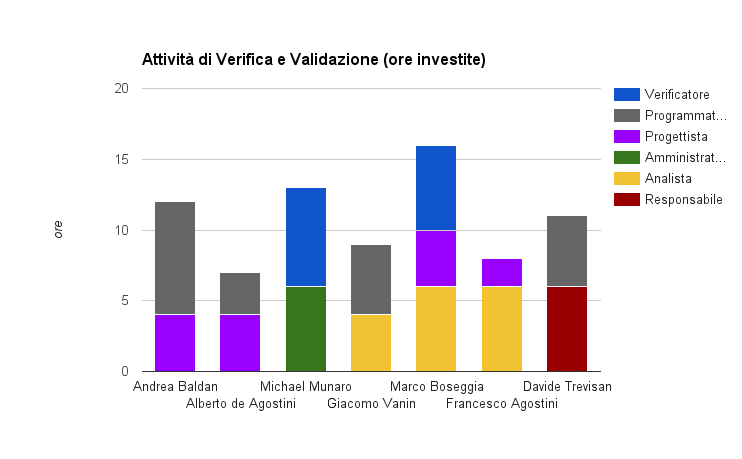
\includegraphics[width=1.2\textwidth,keepaspectratio]{VerificaConInvestimento.png}
    \caption{Ore con investimento, \gloss{attività} di Validazione}
  \end{subfigure}
  \qquad
  \begin{subfigure}[H]{0.47\textwidth}
    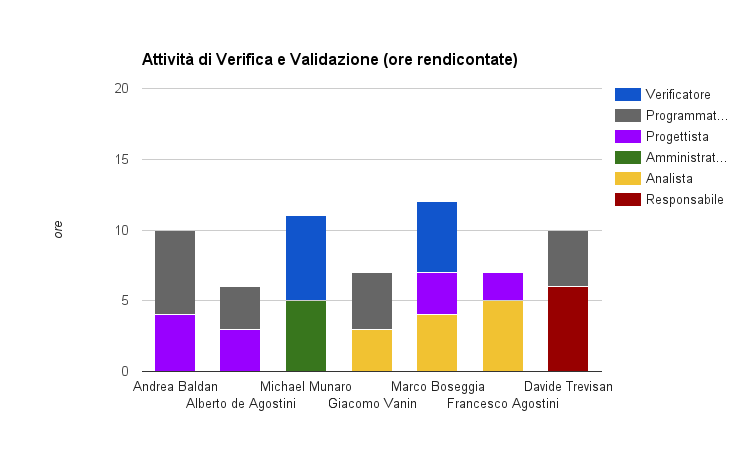
\includegraphics[width=1.2\textwidth,keepaspectratio]{VerificaConRendicontazione.png}
    \caption{Ore con rendicontazione, \gloss{attività} di Validazione}
  \end{subfigure}
\end{figure}

\newpage
\paragraph{Pianificazione temporale}
\begin{figure}[H]
  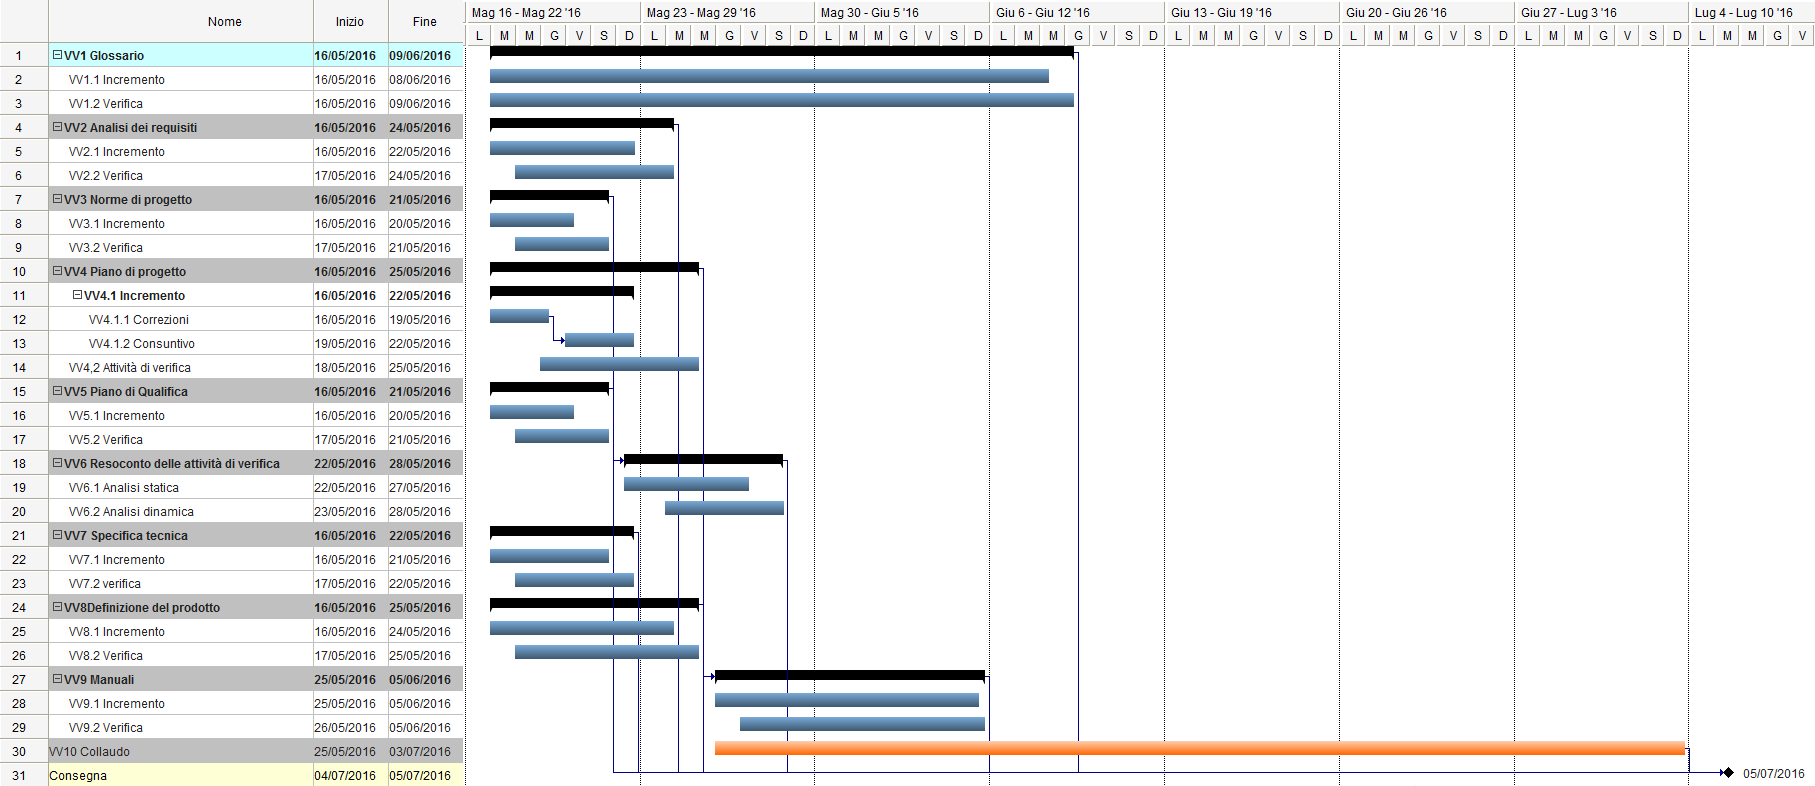
\includegraphics[width=1.0\textwidth, keepaspectratio]{gantt/4-Revisione-Accettazione-gantt-preventivo.png}
  \caption{Gantt preventivo delle \gloss{attività} di Validazione}
\end{figure}

\newpage
\textbf{Distribuzione oraria}
\scriptsize
\begin{center}
  \begin{tabular}{| c | c | c | c |}
    \hline
    \textbf{Id} & \textbf{Nome} & \textbf{Ruolo} & \textbf{Ore}\\
    \hline
    \textbf{VV1} & \textbf{Glossario} & &\\
    \hline
    VV1.1 & Incremento & &\\
    \hline
    VV1.2 & Verifica & Verificatore & 1\\
    \hline
    \textbf{PD2} & \textbf{Analisi dei Requisiti} & &\\
    \hline
    PD2.1 & Incremento & Analista 1 & 5\\
    \hline
    AD2.3 & Verifica & Verificatore 1 & 1\\
    \hline
    \textbf{VV3} & \textbf{Norme di Progetto} & &\\
    \hline
    VV3.1 & Incremento & Amministratore & 4\\
    \hline
    PD3.2 & Verifica & Verificatore 2 & 1\\
    \hline
    \textbf{PD4} & \textbf{Piano di Progetto} & &\\
    \hline
    \textit{PD4.1} & \textit{Incremento} & &\\
    \hline
    PD4.1.1 & Correzioni & Responsabile & 3\\
    \hline
    PD4.1.2 & Consuntivo & Responsabile & 2\\
    \hline
    PD4.2 & Attività di Verifica & Verificatore 2 & 1\\
    \hline
    \textbf{VV5} & \textbf{Piano di Qualifica} & &\\
    \hline
    VV5.1 & Incremento & Analista 2 &3\\
    \hline
    VV5.2 & Verifica & Verificatore 1 &1\\
    \hline
    \textbf{VV6} & \textbf{Resoconto delle \gloss{attività} di verifica} & &\\
    \hline
    VV6.1 & Analisi statica & Verificatore 1 & 2\\
    \hline
    VV6.2 & Analisi dinamica & Verificatore 2 & 1\\
    \hline
    \textbf{VV7} & \textbf{Specifica Tecnica} & &\\
    \hline
    VV7.1 & Incremento & Progettista 2 & 5\\
    \hline
    VV7.2 & Verifica & Verificatore 1 & 1\\
    \hline
    \textbf{VV8} & Definizione del Prodotto & &\\
    \hline
    VV8.1 & Incremento & \multiLineCell[t]{Progettista\\Analista 2} 1 & \multiLineCell[t]{3\\3}\\
    \hline
    VV8.2 & Verifica & Verificatore 2 & 1\\
    \hline
    \textbf{VV9} & \textbf{Manuali} & &\\
    \hline
    VV9.1 & Incremento & \multiLineCell[t]{Analista 2\\Progettista 2} &\multiLineCell[t]{5\\6}\\
    \hline
    VV9.2 & Verifica & Verificatore 2 & 1\\
    \hline
    \textbf{VV10} & Collaudo & \multiLineCell[t]{Programmatore 1\\Programmatore 2\\Amministratore\\Verificatore 1\\Responsabile} & \multiLineCell[t]{11\\10\\2\\2\\1}\\
    \hline
  \end{tabular}
\end{center}
\normalsize
\newpage

\subsubsection{Totale}
Per la durata complessiva del progetto, i componenti ricopriranno i ruoli di progetto secondo la distribuzione seguente:
\begin{center}
  \scriptsize
  \begin{tabular}{| c | p{0.35cm}  p{0.35cm} | p{0.35cm}  p{0.35cm} | p{0.35cm}  p{0.35cm} | p{0.35cm}  p{0.35cm} | p{0.35cm}  p{0.35cm} | p{0.35cm}  p{0.35cm} | p{0.35cm}  p{0.35cm} |}
    \hline
    \textbf{Nome} & \multicolumn{2}{|c|}{\textbf{Res}} & \multicolumn{2}{|c|}{\textbf{An}} & \multicolumn{2}{|c|}{\textbf{Amm}} & \multicolumn{2}{|c|}{\textbf{Pr}} & \multicolumn{2}{|c|}{\textbf{Pt}} & \multicolumn{2}{|c|}{\textbf{Ve}} & \multicolumn{2}{|c|}{\textbf{Tot}}\\
    \hline
    & \textbf{Inv} & \textbf{Ren} & \textbf{Inv} & \textbf{Ren} & \textbf{Inv} & \textbf{Ren} & \textbf{Inv} & \textbf{Ren} & \textbf{Inv} & \textbf{Ren} & \textbf{Inv} & \textbf{Ren} & \textbf{Inv} & \textbf{Ren}\\
    \hline
    Andrea Baldan & 12 & 10 & 15 & 12 & 10 & 8 & 38 & 33 & 22 & 18 & 24 & 20 & 121 & 101\\
    Alberto de Agostini & 12 & 9 & 18 & 14 & 5 & 5 & 38 & 32 & 17 & 15 & 34 & 27 & 124 & 102\\
    Michael Munaro & 10 & 9 & 21 & 17 & 6 & 5 & 18 & 15 & 14 & 11 & 56 & 47 & 125 & 104\\
    Giacomo Vanin & 11 & 10 & 18 & 15 & 6 & 5 & 18 & 16 & 25 & 22 & 43 & 34 & 121 & 102\\
    Marco Boseggia & 8 & 7 & 20 & 16 & 4 & 3 & 29 & 24 & 17 & 15 & 39 & 35 & 117 & 100\\
    Francesco Agostini & 8 & 7 & 19 & 16 & 10 & 8 & 37 & 33 & 10 & 9 & 34 & 30 & 118 & 103\\
    Davide Trevisan & 6 & 6 & 14 & 12 & 4 & 3 & 33 & 28 & 21 & 18 & 41 & 35 & 119 & 102\\
    \hline
  \end{tabular}
\end{center}
\normalsize
I seguenti grafici illustrano le ore investite per Persona suddivise tra ore investite e ore rendicontate durante l'intero progetto:
\begin{figure}[H]
  \begin{subfigure}[H]{0.47\textwidth}
    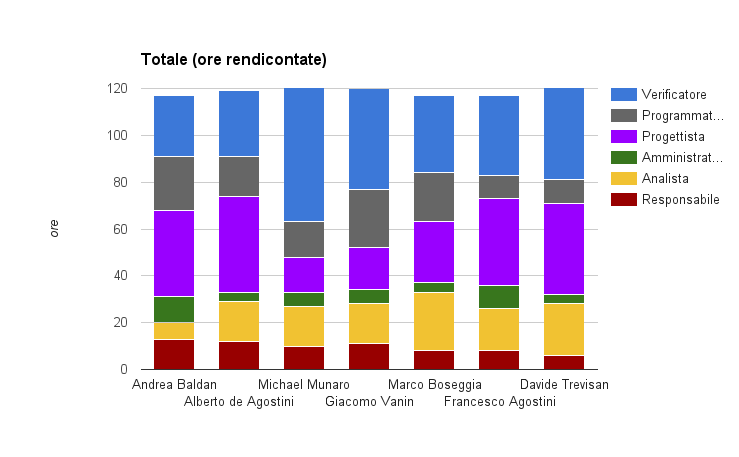
\includegraphics[width=1.2\textwidth,keepaspectratio]{TotaleConInvestimento.png}
    \caption{Ore con investimento totali}
  \end{subfigure}
  \qquad
  \begin{subfigure}[H]{0.47\textwidth}
    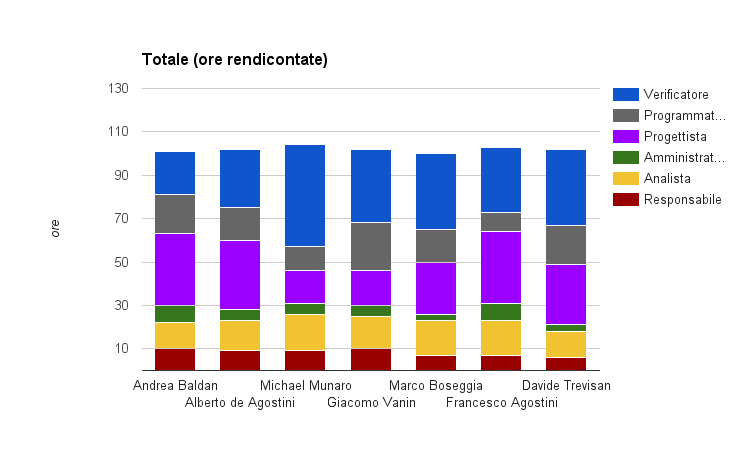
\includegraphics[width=1.2\textwidth,keepaspectratio]{TotaleConRendicontazione.png}
    \caption{Ore con rendicontazione totali}
  \end{subfigure}
\end{figure}

\newpage
\paragraph{Pianificazione temporale}
\begin{figure}[H]
  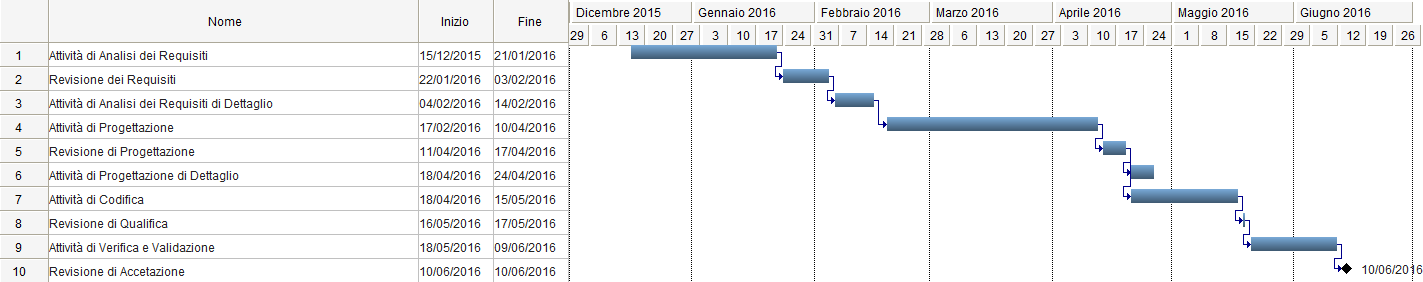
\includegraphics[width=1.0\textwidth, keepaspectratio]{gantt/Gantt-Totale.png}
  \caption{Gantt preventivo di tutto l'arco temporale}
\end{figure}

\newpage
\subsection{Prospetto economico}
In questa sottosezione vengono presentati, per ciascuna \gloss{attività} del progetto identificata
nella sottosezione \ref{sub:fasi}, le ore preventivate di impiego per i ruoli coinvolti.
\subsubsection{Analisi}
Nella fase di Analisi, le ore tra i ruoli sono state divise nel seguente modo:
\begin{center}
  \normalsize
  \begin{tabular}{| c | c | c |}
    \hline
    \multicolumn{3}{|c|}{\textbf{Con investimento}}\\
    \hline
    \textbf{Ruolo} & \textbf{Ore} & \textbf{Costo}\\
    \hline
    Responsabile & 24 & 720\\
    Analista & 73 & 1825\\
    Amministratore & 20 & 400\\
    Progettista & 0 & 0\\
    Programmatore & 0 & 0\\
    Verificatore & 111 & 1665 \\
    \hline
    \textbf{Totale} & 228 & 4610\\
    \hline
  \end{tabular}
  \qquad
  \begin{tabular}{| c | c | c |}
    \hline
    \multicolumn{3}{|c|}{\textbf{Senza investimento}}\\
    \hline
    \textbf{Ruolo} & \textbf{Ore} & \textbf{Costo}\\
    \hline
    Responsabile & 19 & 570\\
    Analista & 62 & 1550\\
    Amministratore & 16 & 320\\
    Progettista & 0 & 0\\
    Programmatore & 0 & 0\\
    Verificatore & 94 & 1410 \\
    \hline
    \textbf{Totale} & 191 & 3850\\
    \hline
  \end{tabular}
\end{center}
I grafici a seguire rappresentano l'influenza di ciascun ruolo sul totale delle ore e dei costi durante l'\gloss{attività} di Analisi.
\begin{figure}[H]
  \begin{subfigure}[H]{0.47\textwidth}
    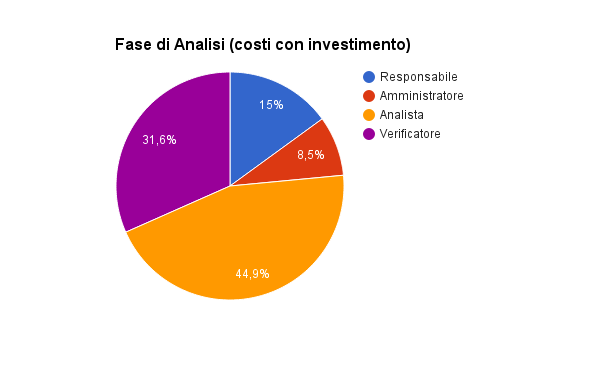
\includegraphics[width=1.2\textwidth,keepaspectratio]{AnalisiCC.png}
    \caption{Costi con investimento, \gloss{attività} di Analisi}
  \end{subfigure}
  \qquad
  \begin{subfigure}[H]{0.47\textwidth}
    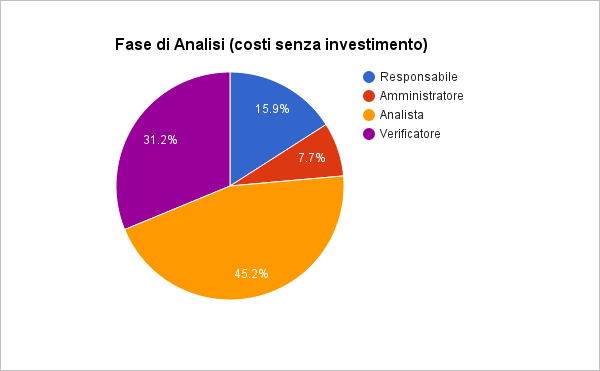
\includegraphics[width=1.2\textwidth,keepaspectratio]{AnalisiSC.png}
    \caption{Costi senza investimento, \gloss{attività} di Analisi}
  \end{subfigure}
\end{figure}
\newpage
\subsubsection{Progettazione}
Durante l'\gloss{attività} di Progettazione, le ore tra i ruoli sono state divise nel seguente modo:
\begin{center}
  \normalsize
  \begin{tabular}{| c | c | c |}
    \hline
    \multicolumn{3}{|c|}{\textbf{Con investimento}}\\
    \hline
    \textbf{Ruolo} & \textbf{Ore} & \textbf{Costo}\\
    \hline
    Responsabile & 19 & 570 \\
    Analista & 29 & 725 \\
    Amministratore & 9 & 180 \\
    Progettista & 94 & 2068\\
    Programmatore & 0 & 0\\
    Verificatore & 56 & 840 \\
    \hline
    \textbf{Totale} & 207 & 4383\\
    \hline
  \end{tabular}
  \qquad
  \begin{tabular}{| c | c | c |}
    \hline
    \multicolumn{3}{|c|}{\textbf{Senza investimento}}\\
    \hline
    \textbf{Ruolo} & \textbf{Ore} & \textbf{Costo}\\
    \hline
    Responsabile & 17 & 510\\
    Analista & 22 & 550\\
    Amministratore & 8 & 160\\
    Progettista & 81 & 1782\\
    Programmatore & 0 & 0\\
    Verificatore & 49 & 735\\
    \hline
    \textbf{Totale} & 177 & 3737 \\
    \hline
  \end{tabular}
\end{center}
I grafici a seguire rappresentano l'influenza di ciascun ruolo sul totale delle ore e dei costi durante l'\gloss{attività} di Progettazione.
\begin{figure}[H]
  \begin{subfigure}[H]{0.47\textwidth}
    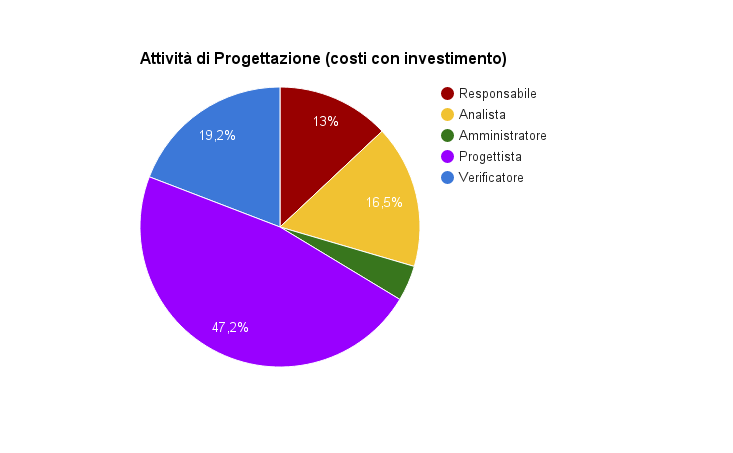
\includegraphics[width=1.2\textwidth,keepaspectratio]{ProgettazioneCC.png}
    \caption{Costi con investimento, \gloss{attività} di Progettazione}
  \end{subfigure}
  \qquad
  \begin{subfigure}[H]{0.47\textwidth}
    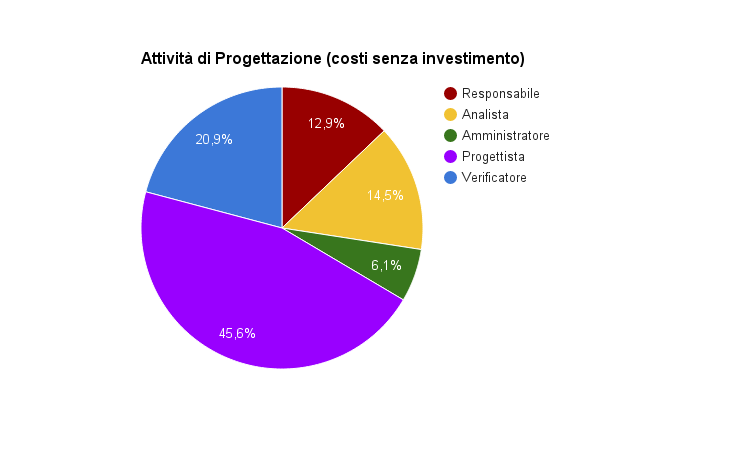
\includegraphics[width=1.2\textwidth,keepaspectratio]{ProgettazioneSC.png}
    \caption{Costi senza investimento, \gloss{attività} di Progettazione}
  \end{subfigure}
\end{figure}
\newpage
\subsubsection{Codifica}
Durante l'\gloss{attività} di Codifica, le ore tra i ruoli sono state divise nel seguente modo:
\begin{center}
  \normalsize
  \begin{tabular}{| c | c | c |}
    \hline
    \multicolumn{3}{|c|}{\textbf{Con investimento}}\\
    \hline
    \textbf{Ruolo} & \textbf{Ore} & \textbf{Costo}\\
    \hline
    Responsabile & 18 & 540 \\
    Analista & 7 & 175\\
    Amministratore & 10 & 200\\
    Progettista & 103 & 2266\\
    Programmatore & 105 & 1575\\
    Verificatore & 91 & 1365\\
    \hline
    \textbf{Totale} & 334 & 6121\\
    \hline
  \end{tabular}
  \qquad
  \begin{tabular}{| c | c | c |}
    \hline
    \multicolumn{3}{|c|}{\textbf{Senza investimento}}\\
    \hline
    \textbf{Ruolo} & \textbf{Ore} & \textbf{Costo}\\
    \hline
    Responsabile & 16 & 480\\
    Analista & 6 & 150\\
    Amministratore & 8 & 160\\
    Progettista & 88 & 1936\\
    Programmatore & 91 & 1365\\
    Verificatore & 74 & 1110\\
    \hline
    \textbf{Totale} & 283 & 5201\\
    \hline
  \end{tabular}
\end{center}
I grafici a seguire rappresentano l'influenza di ciascun ruolo sul totale delle ore e dei costi durante l'\gloss{attività} di Codifica.
\begin{figure}[H]
  \begin{subfigure}[H]{0.47\textwidth}
    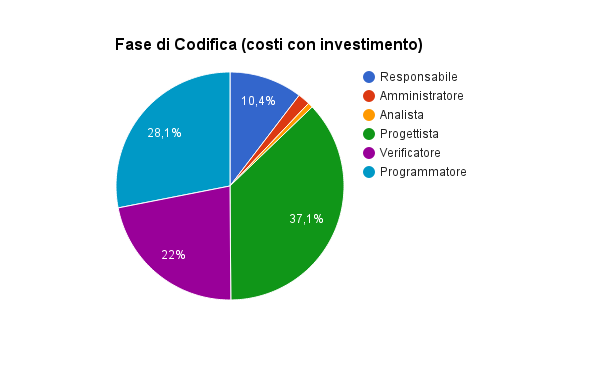
\includegraphics[width=1.2\textwidth,keepaspectratio]{CodificaCC.png}
    \caption{Costi con investimento, \gloss{attività} di Codifica}
  \end{subfigure}
  \qquad
  \begin{subfigure}[H]{0.47\textwidth}
    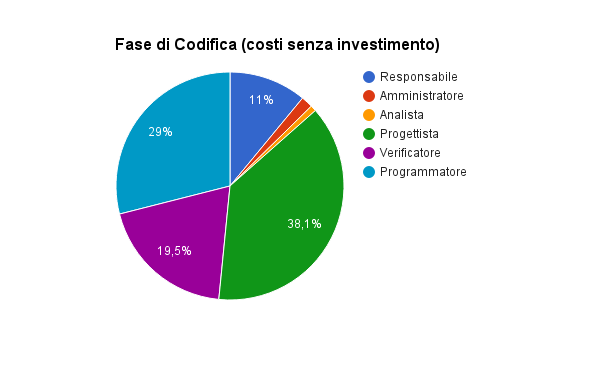
\includegraphics[width=1.2\textwidth,keepaspectratio]{CodificaSC.png}
    \caption{Costi senza investimento, \gloss{attività} di Codifica}
  \end{subfigure}
\end{figure}
\newpage
\subsubsection{Validazione}
Durante le \gloss{attività} di Validazione, le ore tra i ruoli sono state divise nel seguente modo:
\begin{center}
  \normalsize
  \begin{tabular}{| c | c | c |}
    \hline
    \multicolumn{3}{|c|}{\textbf{Con investimento}}\\
    \hline
    \textbf{Ruolo} & \textbf{Ore} & \textbf{Costo}\\
    \hline
    Responsabile & 6 & 180 \\
    Analista & 16 & 400\\
    Amministratore & 6 & 120\\
    Progettista & 14 & 308\\
    Programmatore & 21 & 315\\
    Verificatore & 13 & 195\\
    \hline
    \textbf{Totale} & 76 & 1518\\
    \hline
  \end{tabular}
  \qquad
  \begin{tabular}{| c | c | c |}
    \hline
    \multicolumn{3}{|c|}{\textbf{Senza investimento}}\\
    \hline
    \textbf{Ruolo} & \textbf{Ore} & \textbf{Costo}\\
    \hline
    Responsabile & 6 & 180\\
    Analista & 12 & 300\\
    Amministratore & 5 & 100\\
    Progettista & 12 & 264\\
    Programmatore & 17 & 255\\
    Verificatore & 11 & 165\\
    \hline
    \textbf{Totale} & 63 & 1264\\
    \hline
  \end{tabular}
\end{center}
I grafici a seguire rappresentano l'influenza di ciascun ruolo sul totale delle ore e dei costi durante le \gloss{attività} di Validazione.
\begin{figure}[H]
  \begin{subfigure}[H]{0.47\textwidth}
    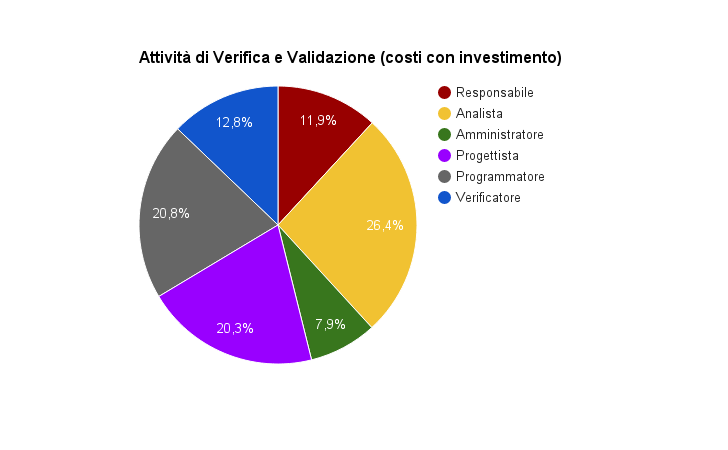
\includegraphics[width=1.2\textwidth,keepaspectratio]{VerificaCC.png}
    \caption{Costi con investimento, \gloss{attività} di Validazione}
  \end{subfigure}
  \qquad
  \begin{subfigure}[H]{0.47\textwidth}
    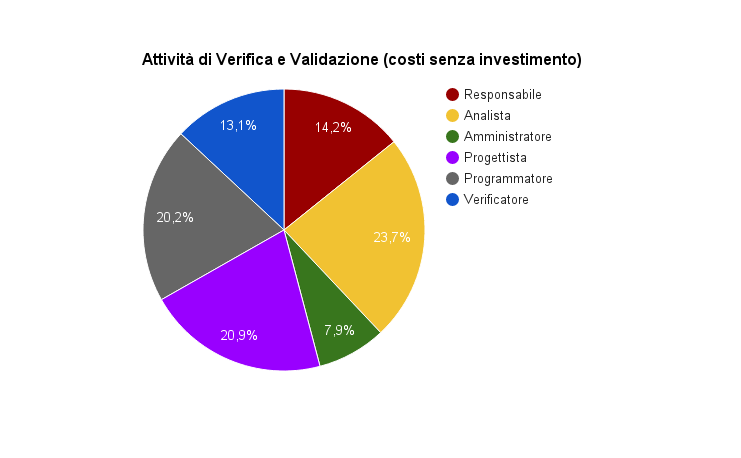
\includegraphics[width=1.2\textwidth,keepaspectratio]{VerificaSC.png}
    \caption{Costi senza investimento, \gloss{attività} di Validazione}
  \end{subfigure}
\end{figure}
\newpage
\subsection{Totale}
Le ore rendicontate totali, previste per la realizzazione del prodotto, senza
investimento sono:
\begin{center}
  \normalsize
  \begin{tabular}{| c | c | c |}
    \hline
    \multicolumn{3}{|c|}{\textbf{Con investimento}}\\
    \hline
    \textbf{Ruolo} & \textbf{Ore} & \textbf{Costo}\\
    \hline
    Responsabile & 67 & 2010 \\
    Analista & 125 & 3125\\
    Amministratore & 45 & 900\\
    Progettista & 211 & 4642\\
    Programmatore & 126 & 1890\\
    Verificatore & 271 & 4065\\
    \hline
    \textbf{Totale} & 845 & 16632\\
    \hline
  \end{tabular}
  \qquad
  \begin{tabular}{| c | c | c |}
    \hline
    \multicolumn{3}{|c|}{\textbf{Senza investimento}}\\
    \hline
    \textbf{Ruolo} & \textbf{Ore} & \textbf{Costo}\\
    \hline
    Responsabile & 58 & 1740\\
    Analista & 102 & 2550\\
    Amministratore & 37 & 740\\
    Progettista & 181 & 3982\\
    Programmatore & 108 & 1620\\
    Verificatore & 228 & 3420\\
    \hline
    \textbf{Totale} & 714 & 14052 \\
    \hline
  \end{tabular}
\end{center}
I grafici a seguire rappresentano l'influenza di ciascun ruolo sul totale delle ore e dei costi complessivi.
\begin{figure}[H]
  \begin{subfigure}[H]{0.47\textwidth}
    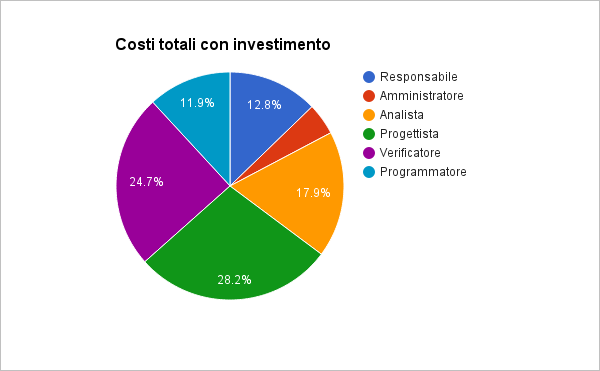
\includegraphics[width=1.2\textwidth,keepaspectratio]{TotaliCC.png}
    \caption{Costi Totali con investimento}
  \end{subfigure}
  \qquad
  \begin{subfigure}[H]{0.47\textwidth}
    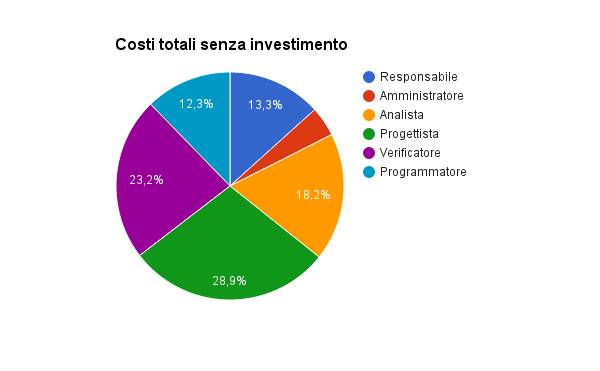
\includegraphics[width=1.2\textwidth,keepaspectratio]{TotaliSC.png}
    \caption{Costi Totali senza investimento}
  \end{subfigure}
\end{figure}

\section{Meccanismi di controllo e rendicontazione}

\subsection{Meccanismi di controllo}
Durante lo sviluppo del nostro ambiente di lavoro si è reso necessario un sistema in grado di permettere:
\begin{itemize}
\item{Pianificazione e controllo le \gloss{attività};}
\item{Flessibilità sulla pianificazione delle \gloss{attività};}
\item{Rendicontazione delle ore spese nelle \gloss{attività}.}
\end{itemize}
\subsubsection{Controllo attività}
Per organizzare il lavoro in maniera ottimale e tenere traccia di ogni singola evoluzione si è deciso di adottare un \gloss{sistema di ticketing}, già descritto nelle \href{run:../Interni/NormeDiProgetto\_v4.0.0.pdf}{Norme di Progetto v4.0.0.}, grazie al quale è
possibile avere un riscontro immediato dello svolgersi di tutte le \gloss{attività} mediante il \gloss{diagramma di Gantt} fornito dal sistema. Esso si aggiorna dinamicamente segnalando graficamente eventuali ritardi nelle \gloss{attività} pianificate, fornendo una visione intuitiva d'insieme dello stato di progetto.
Nello specifico sono evidenziate:
\begin{itemize}
\item{Le \gloss{attività} in ritardo che vengono segnalate in rosso se superata la scadenza prestabilita;}
\item{Lo stato di avanzamento di tutte le \gloss{attività} in corso;}
\item{Le \gloss{attività} già concluse e il tempo reale impiegato.}
\end{itemize}
\subsubsection{Calendario Risorse}
Nel calendario risorse ogni componente del gruppo può segnare impegni e tempo disponibile dedicato
al progetto (come scritto nelle \href{run:../Interni/NormeDiProgetto\_v4.0.0.pdf}{Norme di Progetto v4.0.0.}), in modo che tutto il personale possa organizzare il proprio lavoro in base ai propri
impegni e in sintonia con il lavoro degli altri componenti del gruppo.\\Nel 
\subsubsection{Calendario Attività}
Tutte le \gloss{attività} vengono automaticamente inserite nel calendario dal sistema di ticketing, il quale
indica la data di inizio e la data di fine di ogni \gloss{attività}. Tutti i membri del gruppo vi hanno accesso
e possono monitorare e pianificare il proprio lavoro in base ad esse.
\subsection{Meccanismi di Rendicontazione}
Integrato nel sistema di ticketing vi è un meccanismo di conteggio e misurazione del lavoro svolto
e delle ore impiegate divise per \gloss{attività} e ruolo, esso consente in maniera agevole la rendicontazione
in base a:
\begin{itemize}
\item{Ore di lavoro per \gloss{attività} svolta;}
\item{Ore di lavoro per ruolo.}
\end{itemize}
\newpage

\section{Consuntivo di Periodo}
In questa sezione vengono descritte le spese effettivamente sostenute e suddivise in base ai ruoli,
inoltre nel dettaglio vengono rappresentate per ogni ruolo le ore realmente impiegate. Con questi
dati è possibile stilare un bilancio, che viene calcolato in base alla differenza tra le ore preventivate
e le ore realmente impiegate.
Calcolato il bilancio è possibile trovarsi in tre stati, nello specifico:
\begin{itemize}
\item{\textbf{Bilancio in Positivo} Nel caso le ore preventivate siano superiori di quelle impiegate;}
\item{\textbf{Bilancio in Negativo} Nel caso le ore impiegate siano superiori a quelle preventivate;}
\item{\textbf{Bilancio in Pari} Nel caso le ore preventivate corrispondano a quelle realmente impiegate.}
\end{itemize}
\subsection{Analisi}
Viene di seguito riportato il consuntivo relativo alla fase di analisi e riportate per ogni ruolo lo
scarto tra le ore in preventivo e le ore impiegate formando un bilancio per ciascuno di essi.
\begin{center}
  \normalsize
  \begin{tabular}{| c | c | c |}
    \hline
    \textbf{Ruolo} & \textbf{Ore} & \textbf{Costo}\\
    \hline
    Responsabile & -1 & -30 \\
    Analista & -2 & -50\\
    Amministratore & -1 & -20\\
    Progettista & 0 & 0\\
    Programmatore & 0 & 0\\
    Verificatore & +1 & +15\\
    \hline
    \textbf{Totale} & -3 & -85\\
    \hline
  \end{tabular}
\end{center}

\subsubsection{Conclusioni}
Le \gloss{attività} pianificate si sono svolte sforando di alcune ore rispetto a quanto pianificato, con un bilancio in negativo di \textbf{\euro{} 85} che rientra nelle metriche decise nel \href{run:PianoDiQualifica\_v4.0.0.pdf}{Piano di Qualifica v4.0.0}.

\subsection{Progettazione}
Viene di seguito riportato il consuntivo temporale ed economico relativo alla fase di progettazione. Gli indici riportati rappresentano lo schedule variance e il budget variance calcolati alla fine del periodo riservato per questa fase di progetto. I valori dello schedule variance sono stati calcolati (intermedi alla durata di questo periodo) e salvati nel forum del gruppo e si è scelto di non riportarli in questo documento per evitare verbosità ritenendo opportuno far conoscere lo schedule variance totale dell'intera fase.\\
Di seguito viene riportata in tabella il numero di ore di ritardo o di anticipo per ruolo e il relativo costo o risparmio.
\begin{center}
  \normalsize
  \begin{tabular}{| c | c | c |}
    \hline
    \textbf{Ruolo} & \textbf{Ore (SV)} & \textbf{Costo (BV)}\\
    \hline
    Responsabile & -1 & -30 \\
    Analista & -8 & -200\\
    Amministratore & 0 & 0\\
    Progettista & -4 & -88\\
    Programmatore & 0 & 0\\
    Verificatore & -5 & -75\\
    \hline
    \textbf{Totale} & -18 & -393\\
    \hline
  \end{tabular}
\end{center}

\subsubsection{Conclusioni}
Le \gloss{attività} pianificate si sono svolte sforando di parecchie ore rispetto a quanto pianificato, principalmente questo è stato dovuto a diversi errori fatti durante le attività di analisi della scorsa fase, il gruppo ha dovuto così lavorare più ore del previsto per correggere tali errori e procedere con la progettazione.\\Infine quindi abbiamo ottenuto un bilancio orario in negativo di \textbf{18 ore} e di \textbf{\euro{} 393}.\\ Entrambi i valori sebbene negativi rientrano nei range di accettazione scritti nel \href{run:PianoDiQualifica\_v4.0.0.pdf}{Piano di Qualifica v4.0.0}.

\subsection{Codifica}
Viene di seguito riportato il consuntivo temporale ed economico relativo alla 
fase di codifica. Gli indici riportati rappresentano lo schedule variance e il 
budget variance calcolati alla fine del periodo riservato per questa fase di 
progetto.\\I valori di schedule variance e budget variance intermedi alla 
durata di questo periodo sono stati inseriti nel documento \href{run:./Esterno/PianoDiQualifica\_v4.0.0.pdf}{Piano di Qualifica v4.0.0.}.\\Di seguito 
viene riportato in tabella il numero di ore di ritardo o di anticipo per 
ruolo e il relativo costo o risparmio.
\begin{center}
  \normalsize
  \begin{tabular}{| c | c | c |}
    \hline
    \textbf{Ruolo} & \textbf{Ore (SV)} & \textbf{Costo (BV)}\\
    \hline
    Responsabile & +5 & +150\\ %30
    Analista & 0 & 0\\ %25
    Amministratore & +2 & +40\\ %20
    Progettista & -1 & -22\\ %22
    Programmatore & -1 & -15\\ %15
    Verificatore & +2 & +30\\ %15    
    \hline
    \textbf{Totale} & +7 & +203\\    
    \hline
  \end{tabular}
\end{center}

\subsubsection{Conclusioni}
Le \gloss{attività} pianificate si sono svolte con un risparmio di ore e 
denaro. Una delle motivazioni di questo risparmio deriva dalle modifiche 
architetturali effettuate su consiglio del \textit{committente} e 
\textit{proponente}.\\Possiamo vedere che il bilancio finale di questo periodo 
è stato in positivo di \textbf{7 ore} e di \textbf{\euro{} 203}.\\

\subsection{Validazione}
Viene di seguito riportato il consuntivo temporale ed economico relativo alla 
fase di validazione. Gli indici riportati rappresentano lo schedule variance 
e il budget variance calcolati alla fine del periodo riservato per questa 
fase di progetto.\\I valori di schedule variance e budget variance intermedi 
alla durata di questo periodo sono stati inseriti nel documento 
\href{run:./Esterno/PianoDiQualifica\_v4.0.0.pdf}{Piano di Qualifica v4.0.0.}.\\Di seguito viene riportato in tabella il numero di ore di ritardo o di 
anticipo per ruolo e il relativo costo o risparmio.
\begin{center}
  \normalsize
  \begin{tabular}{| c | c | c |}
    \hline
    \textbf{Ruolo} & \textbf{Ore (SV)} & \textbf{Costo (BV)}\\
    \hline
    Responsabile & +4 & +120\\ %30 %TODO fare sta tabella
    Analista & +4 & +100\\ %25
    Amministratore & +3 & +60\\ %20
    Progettista & +4 & +88\\ %22
    Programmatore & -3 & -45\\ %15
    Verificatore & +1 & 15\\ %15    
    \hline
    \textbf{Totale} & +13 & +338\\    
    \hline
  \end{tabular}
\end{center}

\subsubsection{Conclusioni}
Le \gloss{attività} pianificate si sono svolte con un risparmio di ore e 
denaro. Una delle motivazioni di questo risparmio deriva dalle modifiche 
architetturali effettuate su consiglio del \textit{committente} e 
\textit{proponente}.\\Possiamo vedere che il bilancio finale di questo periodo 
è stato in positivo di \textbf{13} e di \textbf{\euro{} 338}.\\

\subsection{Totale}
Viene di seguito riportato il consuntivo temporale ed economico relativo alla 
totalità della durata del progetto. Gli indici riportati rappresentano lo 
schedule variance e il budget variance calcolati alla fine dell'intero periodo 
di durata del progetto.\\Di seguito viene riportato in tabella il numero di ore 
di ritardo o di anticipo per ruolo e il relativo costo o risparmio.

\begin{center}
  \normalsize
  \begin{tabular}{| c | c | c |}
    \hline
    \textbf{Ruolo} & \textbf{Ore (SV)} & \textbf{Costo (BV)}\\
    \hline
    Responsabile & +7 & +210\\ %30    k
    Analista & -6 & -150\\ %25        k
    Amministratore & +4 & +80\\ %20   k
    Progettista & -1 & -22\\ %22      k
    Programmatore & -4 & -60\\ %15    k
    Verificatore & -2 & -30\\ %15     k
    \hline
    \textbf{Totale} & -2 & +28\\    
    \hline
  \end{tabular}
\end{center}

Le \gloss{attività} 
Nella seguente tabella viene riportata per ogni membro del gruppo le ore 
preventivate e quelle realmente lavorate. il numero tra parentesi tonde 
rappresenta il numero di ore preventivate mentre il numero senza parentesi 
indica il numero di ore realmente lavorate.\\
\begin{center}
  \begin{tabular}{| c | l | l | l | l | l | l | l |}
    \hline
    \multirow{2}{*}{\textbf{Nominativo}} & \multicolumn{6}{c|}{\textbf{Ore per ruolo}} & \multirow{2}{*}{\textbf{Ore totali}} \\
    \cline{2-7}
        & \textbf{Re} & \textbf{Am} & \textbf{An} & \textbf{Pt} & \textbf{Pg} & \textbf{Ve} & \\
    \hline
    Agostini Francesco  & (7) 5   & (8) 10 & (16) 16 & (33) 33 & (9)  9 & (30) 30 & (103) 103\\
    \hline
    Baldan Andrea       & (10) 10 & (8) 9 & (12) 12 & (33) 34 & (18) 20 & (20) 20 & (101) 105\\
    \hline
    Boseggia Marco      & (7) 7   & (3) 3 & (16) 17 & (24) 25 & (15) 16 & (35) 37 & (100) 105\\
    \hline
    De Agostini Alberto & (9) 8   & (5) 4 & (14) 15 & (32) 32 & (15) 16 & (27) 30 & (102) 105\\
    \hline
    Munaro Michael      & (9) 8   & (5) 4 & (17) 20 & (15) 15 & (11) 11 & (42) 46 & (104) 104\\
    \hline
    Trevisan Davide     & (6) 4   & (3) 2 & (12) 12 & (28) 27 & (18) 12 & (35) 28 & (102) 85\\
    \hline
    Vanin Giacomo       & (10) 9  & (5) 2 & (15) 16 & (16) 16 & (22) 28 & (34) 34 & (102) 105\\
    \hline
  \end{tabular}
\end{center}

\subsubsection{Conclusioni}
Le \gloss{attività} pianificate si sono svolte con un dispendio di ore ma con un risparmio di 
denaro. Una delle motivazioni di questo risparmio deriva dal buon punto in cui il gruppo era 
riuscito ad arrivare in sede di RQ. Il numero di ore di lavoro totale è maggiore di quello 
preventivato dal gruppo ma di poco raggiungendo quindi un punto di arrivo soddisfacente per il gruppo.\\Possiamo vedere che il bilancio finale del periodo complessivo della durata del progetto 
è stato in negativo di \textbf{2} ore e in positivo di \textbf{\euro{} 28}.\\

\section{Organigramma}
\subsection{Accettazione componenti}
\begin{center}
  \begin{tabular}{|l | l | p{4cm} |}
    \hline
    Nome & Data & Firme \\
    \hline
    Alberto De Agostini & 2015-12-18 & 
\includegraphics[height=1cm,keepaspectratio]{Signs/elettroCardiogramma.png} \\
    Andrea Giacomo Baldan & 2015-12-18 &
\includegraphics[height=1cm,keepaspectratio]{Signs/andrea.png} \\
    Marco Boseggia & 2015-12-18 &
\includegraphics[height=1cm,keepaspectratio]{Signs/marco.png} \\
    Giacomo Vanin & 2015-12-18 & 
\includegraphics[height=1cm,keepaspectratio]{Signs/giacomo.png}\\
    Michael Munaro & 2015-12-18 &
\includegraphics[height=1cm,keepaspectratio]{Signs/michael.png}\\
    Davide Trevisan & 2015-12-18 &
\includegraphics[height=0.9cm,keepaspectratio]{Signs/davide.png}\\
    Francesco Agostini & 2015-12-18 &
\includegraphics[height=1cm,keepaspectratio]{Signs/francesco.png}\\
    \hline
  \end{tabular}
\end{center}
\subsection{Componenti}
\begin{center}
  \begin{tabular}{|l | l | l |}
    \hline
    Nome & Matricola & Email \\
    \hline
    Alberto De Agostini & 579021 & albertodeagostini88@gmail.com\\
    Andrea Giacomo Baldan & 579117 & a.g.baldan@gmail.com\\
    Marco Boseggia & 1044608 & boseggiam91@gmail.com\\
    Giacomo Vanin & 1026988 & giacomo.vanin92@gmail.com\\
    Michael Munaro & 1049522 & munaro.michael@gmail.com\\
    Davide Trevisan & 1070686 & trevisan.davide94@libero.it\\
    Francesco Agostini & 1051519 & francesco.agostini.93@gmail.com\\
    \hline
  \end{tabular}
\end{center}
\newpage
\appendix
\listoftables
\listoffigures
\end{document}
